\documentclass[11pt]{article}
\usepackage[margin=1in]{geometry}
\usepackage[T1]{fontenc}
\usepackage{lmodern}
\usepackage{amsmath,amssymb,booktabs,icomma,array,graphicx}
\usepackage[round]{natbib}
\usepackage{placeins}
\usepackage[hidelinks]{hyperref}

% Result numbers. Generated by `crew.py numbers`; never typed by hand.
% Generated by `crew.py numbers` from claims.jsonl. Do not edit by hand.
% Each macro is a number taken from a logged run; see claims.jsonl.
\newcommand{\PrimaryEffect}{-10}  % primary-effect
\newcommand{\PrimaryCILow}{-358}  % primary-ci-low
\newcommand{\PrimaryCIHigh}{338}  % primary-ci-high
\newcommand{\PrimarySE}{178}  % primary-se
\newcommand{\PrimaryP}{0.956}  % primary-p
\newcommand{\PrimaryCINinetyLow}{-302}  % primary-ci90-low
\newcommand{\PrimaryCINinetyHigh}{282}  % primary-ci90-high
\newcommand{\PrimaryTOSTP}{0.004}  % primary-tost-p
\newcommand{\PrimaryMinMargin}{302}  % primary-min-margin
\newcommand{\EquivMargin}{483.47}  % equiv-margin
\newcommand{\PrimaryRelEffect}{-0.1}  % primary-rel-effect
\newcommand{\PrimaryRelCILow}{-4.3}  % primary-rel-ci-low
\newcommand{\PrimaryRelCIHigh}{4.1}  % primary-rel-ci-high
\newcommand{\PrimaryCFMean}{7,940}  % primary-cf-mean
\newcommand{\PrimaryTreatedMean}{7,930}  % primary-treated-mean
\newcommand{\PrimaryEffectOverMargin}{-0.02}  % primary-effect-over-margin
\newcommand{\PrimaryN}{4,000}  % primary-n
\newcommand{\PrimaryNTreated}{1,621}  % primary-n-treated
\newcommand{\PrimaryNControl}{2,379}  % primary-n-control
\newcommand{\PrimaryNClipped}{0}  % primary-n-clipped
\newcommand{\OverlapShareOutside}{0.033}  % overlap-share-outside
\newcommand{\OverlapTreatedAboveNineTenths}{0.000}  % overlap-treated-above-09
\newcommand{\SecEarnNextEffect}{-112}  % sec-re79-effect
\newcommand{\SecEarnNextSE}{196}  % sec-re79-se
\newcommand{\SecEarnNextCILow}{-495}  % sec-re79-ci-low
\newcommand{\SecEarnNextCIHigh}{272}  % sec-re79-ci-high
\newcommand{\SecEarnNextP}{0.568}  % sec-re79-p
\newcommand{\SecEarnNextPRW}{0.744}  % sec-re79-p-rw
\newcommand{\SecEarnNextMaxTLow}{-596}  % sec-re79-maxt-low
\newcommand{\SecEarnNextMaxTHigh}{373}  % sec-re79-maxt-high
\newcommand{\SecEmployedEffect}{1.0}  % sec-employed78-effect
\newcommand{\SecEmployedSE}{1.4}  % sec-employed78-se
\newcommand{\SecEmployedCILow}{-1.7}  % sec-employed78-ci-low
\newcommand{\SecEmployedCIHigh}{3.7}  % sec-employed78-ci-high
\newcommand{\SecEmployedP}{0.465}  % sec-employed78-p
\newcommand{\SecEmployedPRW}{0.744}  % sec-employed78-p-rw
\newcommand{\SecEmployedMaxTLow}{-2.4}  % sec-employed78-maxt-low
\newcommand{\SecEmployedMaxTHigh}{4.4}  % sec-employed78-maxt-high
\newcommand{\SecHoursEffect}{48.2}  % sec-hours78-effect
\newcommand{\SecHoursSE}{26.3}  % sec-hours78-se
\newcommand{\SecHoursCILow}{-3.4}  % sec-hours78-ci-low
\newcommand{\SecHoursCIHigh}{99.8}  % sec-hours78-ci-high
\newcommand{\SecHoursP}{0.067}  % sec-hours78-p
\newcommand{\SecHoursPRW}{0.204}  % sec-hours78-p-rw
\newcommand{\SecHoursMaxTLow}{-17.0}  % sec-hours78-maxt-low
\newcommand{\SecHoursMaxTHigh}{113.5}  % sec-hours78-maxt-high
\newcommand{\SecBenefitsEffect}{87}  % sec-benefits78-effect
\newcommand{\SecBenefitsSE}{43}  % sec-benefits78-se
\newcommand{\SecBenefitsCILow}{3}  % sec-benefits78-ci-low
\newcommand{\SecBenefitsCIHigh}{171}  % sec-benefits78-ci-high
\newcommand{\SecBenefitsP}{0.044}  % sec-benefits78-p
\newcommand{\SecBenefitsPRW}{0.166}  % sec-benefits78-p-rw
\newcommand{\SecBenefitsMaxTLow}{-20}  % sec-benefits78-maxt-low
\newcommand{\SecBenefitsMaxTHigh}{194}  % sec-benefits78-maxt-high
\newcommand{\SecWellbeingEffect}{0.06}  % sec-wellbeing78-effect
\newcommand{\SecWellbeingSE}{0.07}  % sec-wellbeing78-se
\newcommand{\SecWellbeingCILow}{-0.08}  % sec-wellbeing78-ci-low
\newcommand{\SecWellbeingCIHigh}{0.21}  % sec-wellbeing78-ci-high
\newcommand{\SecWellbeingP}{0.383}  % sec-wellbeing78-p
\newcommand{\SecWellbeingPRW}{0.744}  % sec-wellbeing78-p-rw
\newcommand{\SecWellbeingMaxTLow}{-0.12}  % sec-wellbeing78-maxt-low
\newcommand{\SecWellbeingMaxTHigh}{0.24}  % sec-wellbeing78-maxt-high
\newcommand{\SecMaxTCrit}{2.477}  % sec-maxt-crit
\newcommand{\SecNDetected}{0}  % sec-n-detected
\newcommand{\SecWellbeingEffectSD}{0.036}  % sec-wellbeing78-effect-sd
\newcommand{\SecWellbeingControlSD}{1.78}  % sec-wellbeing78-control-sd
\newcommand{\SelectEarnPriorEffect}{-3,541}  % select-re75-effect
\newcommand{\SelectEarnPriorCILow}{-3,878}  % select-re75-ci-low
\newcommand{\SelectEarnPriorCIHigh}{-3,204}  % select-re75-ci-high
\newcommand{\SelectEarnPriorOverMargin}{-7.3}  % select-re75-over-margin
\newcommand{\TrimEffect}{36}  % trim-effect
\newcommand{\TrimCILow}{-300}  % trim-ci-low
\newcommand{\TrimCIHigh}{371}  % trim-ci-high
\newcommand{\TrimN}{3,867}  % trim-n
\newcommand{\TrimCINinetyLow}{-246}  % trim-ci90-low
\newcommand{\TrimCINinetyHigh}{317}  % trim-ci90-high
\newcommand{\CovsetAEffect}{-32}  % covset-a-effect
\newcommand{\CovsetACILow}{-370}  % covset-a-ci-low
\newcommand{\CovsetACIHigh}{307}  % covset-a-ci-high
\newcommand{\CovsetAN}{4,000}  % covset-a-n
\newcommand{\CovsetACINinetyLow}{-316}  % covset-a-ci90-low
\newcommand{\CovsetACINinetyHigh}{253}  % covset-a-ci90-high
\newcommand{\CovsetBEffect}{-139}  % covset-b-effect
\newcommand{\CovsetBCILow}{-494}  % covset-b-ci-low
\newcommand{\CovsetBCIHigh}{215}  % covset-b-ci-high
\newcommand{\CovsetBN}{4,000}  % covset-b-n
\newcommand{\CovsetBCINinetyLow}{-437}  % covset-b-ci90-low
\newcommand{\CovsetBCINinetyHigh}{158}  % covset-b-ci90-high
\newcommand{\LearnerLinearEffect}{-116}  % learner-linear-effect
\newcommand{\LearnerLinearCILow}{-450}  % learner-linear-ci-low
\newcommand{\LearnerLinearCIHigh}{218}  % learner-linear-ci-high
\newcommand{\LearnerLinearN}{4,000}  % learner-linear-n
\newcommand{\LearnerLinearCINinetyLow}{-396}  % learner-linear-ci90-low
\newcommand{\LearnerLinearCINinetyHigh}{165}  % learner-linear-ci90-high
\newcommand{\LearnerRFEffect}{-10}  % learner-rf-effect
\newcommand{\LearnerRFCILow}{-358}  % learner-rf-ci-low
\newcommand{\LearnerRFCIHigh}{338}  % learner-rf-ci-high
\newcommand{\LearnerRFN}{4,000}  % learner-rf-n
\newcommand{\LearnerRFCINinetyLow}{-302}  % learner-rf-ci90-low
\newcommand{\LearnerRFCINinetyHigh}{282}  % learner-rf-ci90-high
\newcommand{\DiffSeventyFourEffect}{-1,087}  % diff74-effect
\newcommand{\DiffSeventyFourCILow}{-1,496}  % diff74-ci-low
\newcommand{\DiffSeventyFourCIHigh}{-678}  % diff74-ci-high
\newcommand{\DiffSeventyFourN}{4,000}  % diff74-n
\newcommand{\DiffSeventyFourCINinetyLow}{-1,430}  % diff74-ci90-low
\newcommand{\DiffSeventyFourCINinetyHigh}{-743}  % diff74-ci90-high
\newcommand{\OLSEffect}{-127}  % ols-effect
\newcommand{\OLSCILow}{-434}  % ols-ci-low
\newcommand{\OLSCIHigh}{181}  % ols-ci-high
\newcommand{\OLSN}{4,000}  % ols-n
\newcommand{\IPWEffect}{-191}  % ipw-effect
\newcommand{\IPWCILow}{-521}  % ipw-ci-low
\newcommand{\IPWCIHigh}{139}  % ipw-ci-high
\newcommand{\IPWN}{4,000}  % ipw-n
\newcommand{\IPWCINinetyLow}{-468}  % ipw-ci90-low
\newcommand{\IPWCINinetyHigh}{86}  % ipw-ci90-high
\newcommand{\TrimNTreated}{1,611}  % trim-n-treated
\newcommand{\TrimNDropped}{133}  % trim-n-dropped
\newcommand{\SensRsqMargin}{0.060}  % sens-r2-margin
\newcommand{\SensTargetMargin}{483}  % sens-target-margin
\newcommand{\SensRsqZero}{0.042}  % sens-r2-zero
\newcommand{\SensTargetZero}{338}  % sens-target-zero
\newcommand{\SensRsqEquiv}{0.023}  % sens-r2-equiv
\newcommand{\SensTargetEquiv}{181}  % sens-target-equiv
\newcommand{\SensBenchAgeRsqD}{0.010}  % sens-bench-age-r2d
\newcommand{\SensBenchAgeRsqY}{0.025}  % sens-bench-age-r2y
\newcommand{\SensBenchAgeBias}{128}  % sens-bench-age-bias
\newcommand{\SensBenchEducRsqD}{0.024}  % sens-bench-educ-r2d
\newcommand{\SensBenchEducRsqY}{0.010}  % sens-bench-educ-r2y
\newcommand{\SensBenchEducBias}{126}  % sens-bench-educ-bias
\newcommand{\SensBenchMarriedRsqD}{0.000}  % sens-bench-married-r2d
\newcommand{\SensBenchMarriedRsqY}{0.001}  % sens-bench-married-r2y
\newcommand{\SensBenchMarriedBias}{6}  % sens-bench-married-bias
\newcommand{\SensBenchUrbanRsqD}{0.000}  % sens-bench-urban-r2d
\newcommand{\SensBenchUrbanRsqY}{0.001}  % sens-bench-urban-r2y
\newcommand{\SensBenchUrbanBias}{5}  % sens-bench-urban-bias
\newcommand{\SensBenchRegionRsqD}{0.000}  % sens-bench-region-r2d
\newcommand{\SensBenchRegionRsqY}{0.000}  % sens-bench-region-r2y
\newcommand{\SensBenchRegionBias}{0}  % sens-bench-region-bias
\newcommand{\SensBenchChildrenRsqD}{0.000}  % sens-bench-children-r2d
\newcommand{\SensBenchChildrenRsqY}{0.000}  % sens-bench-children-r2y
\newcommand{\SensBenchChildrenBias}{1}  % sens-bench-children-bias
\newcommand{\SensBenchHealthRsqD}{0.002}  % sens-bench-health-r2d
\newcommand{\SensBenchHealthRsqY}{0.000}  % sens-bench-health-r2y
\newcommand{\SensBenchHealthBias}{6}  % sens-bench-health-bias
\newcommand{\SensBenchEarnSeventyFourRsqD}{0.010}  % sens-bench-earn74-r2d
\newcommand{\SensBenchEarnSeventyFourRsqY}{0.066}  % sens-bench-earn74-r2y
\newcommand{\SensBenchEarnSeventyFourBias}{204}  % sens-bench-earn74-bias
\newcommand{\SensBenchEarnSeventyFiveRsqD}{0.189}  % sens-bench-earn75-r2d
\newcommand{\SensBenchEarnSeventyFiveRsqY}{0.237}  % sens-bench-earn75-r2y
\newcommand{\SensBenchEarnSeventyFiveBias}{1,716}  % sens-bench-earn75-bias
\newcommand{\SensTauZero}{-127}  % sens-tau00
\newcommand{\SensSigmaZero}{4,407}  % sens-sigma-zero
\newcommand{\MissingEarnTreated}{0}  % missing-re78-treated
\newcommand{\InvalidEarnTreated}{0}  % invalid-re78-treated
\newcommand{\MissingEarnControl}{0}  % missing-re78-control
\newcommand{\InvalidEarnControl}{0}  % invalid-re78-control
\newcommand{\MissingEarnNextTreated}{0}  % missing-re79-treated
\newcommand{\InvalidEarnNextTreated}{0}  % invalid-re79-treated
\newcommand{\MissingEarnNextControl}{0}  % missing-re79-control
\newcommand{\InvalidEarnNextControl}{0}  % invalid-re79-control
\newcommand{\MissingEmployedTreated}{0}  % missing-employed78-treated
\newcommand{\InvalidEmployedTreated}{0}  % invalid-employed78-treated
\newcommand{\MissingEmployedControl}{0}  % missing-employed78-control
\newcommand{\InvalidEmployedControl}{0}  % invalid-employed78-control
\newcommand{\MissingHoursTreated}{0}  % missing-hours78-treated
\newcommand{\InvalidHoursTreated}{0}  % invalid-hours78-treated
\newcommand{\MissingHoursControl}{0}  % missing-hours78-control
\newcommand{\InvalidHoursControl}{0}  % invalid-hours78-control
\newcommand{\MissingBenefitsTreated}{0}  % missing-benefits78-treated
\newcommand{\InvalidBenefitsTreated}{0}  % invalid-benefits78-treated
\newcommand{\MissingBenefitsControl}{0}  % missing-benefits78-control
\newcommand{\InvalidBenefitsControl}{0}  % invalid-benefits78-control
\newcommand{\MissingWellbeingTreated}{0}  % missing-wellbeing78-treated
\newcommand{\InvalidWellbeingTreated}{0}  % invalid-wellbeing78-treated
\newcommand{\MissingWellbeingControl}{0}  % missing-wellbeing78-control
\newcommand{\InvalidWellbeingControl}{0}  % invalid-wellbeing78-control


% Magnitude of a negative macro value (drops the leading minus sign of the macro's text).
\def\absvalaux-#1\relax{#1}
\newcommand{\absval}[1]{\expandafter\absvalaux#1\relax}

\setlength{\emergencystretch}{2em}
\setlength{\belowcaptionskip}{6pt}
\renewcommand{\topfraction}{0.9}
\renewcommand{\bottomfraction}{0.8}
\renewcommand{\textfraction}{0.07}
\renewcommand{\floatpagefraction}{0.8}
\newcommand{\var}[1]{\texttt{#1}}
\newcommand{\ci}[2]{$[#1, #2]$}

\title{Did a Job-Training Program Raise Participants' Earnings?\\
A Pre-Specified Observational Evaluation on Synthetic Data}
\author{Bryce Wang (human PI) \\ \small Drafted with Free-Research-Crew; see the AI-use statement.}
\date{\today}

\begin{document}
\maketitle

\begin{abstract}
We estimate the average effect on the treated (ATT) of enrolling in a voluntary 1976--77
job-training program on 1978 earnings, in a synthetic extract of $\PrimaryN$ adults of
whom $\PrimaryNTreated$ enrolled. The data are synthetic, and no claim is made about any
real program. The estimand, the eleven conditioning covariates, the closed list of outcomes,
their multiple-testing corrections and an equivalence margin $M$ (10\% of enrolees' mean
1975 earnings, $M = \EquivMargin$ nominal dollars) were all fixed before any analysis used an
outcome value; before that, two counts-only runs read the outcome columns to count missing
and out-of-range entries. The cross-fitted doubly robust (AIPW) estimate of the ATT is $\PrimaryEffect$ dollars,
with 95\% confidence interval \ci{\PrimaryCILow}{\PrimaryCIHigh}, or $\PrimaryRelEffect$\%
of enrolees' estimated counterfactual mean. A zero ATT is not rejected ($p = \PrimaryP$).
Under unconfoundedness given the eleven covariates, the 90\% interval
\ci{\PrimaryCINinetyLow}{\PrimaryCINinetyHigh} lies inside $\pm M$ (equivalence test
$p = \PrimaryTOSTP$). This conclusion is not robust to unobserved selection as strong as
the observed selection on 1975 earnings: in the pre-specified
sensitivity analysis, a confounder that strong would move the estimate by up to
$\SensBenchEarnSeventyFiveBias$ dollars, so the result could be produced by unobserved
selection of that strength, and an unobserved 1976 earnings shock is plausibly at least
that strongly related to enrolment. The equivalence conclusion is also not robust to a
confounder as strong as 1974 earnings. A pre-specified conditional difference-in-differences
estimate from 1974, which rests on a different assumption, is $\DiffSeventyFourEffect$
dollars \ci{\DiffSeventyFourCILow}{\DiffSeventyFourCIHigh}, with its whole 90\% interval
below $-M$. None of five secondary outcomes is detected after Romano--Wolf adjustment.
\end{abstract}

\section{Introduction}

Whether voluntary job training raises the earnings of the people who take it is one of the
best-studied questions in applied economics, and also one of the questions on which
non-experimental methods have the most uneven record. \citet{lalonde1986} showed that
non-experimental estimators applied to the National Supported Work (NSW) demonstration
often failed to replicate the experimental estimates, even when they passed conventional
specification tests. Propensity-score stratification and matching later produced estimates
close to the experimental benchmark by using only comparison units similar to the treated
\citep{dehejia1999,dehejia2002}, but those estimates turned out to be highly sensitive to the
variables included in the score and to the analysis sample
\citep{smith2005}, and \citet{dehejia2005} argued that the specification must be chosen
separately for each treatment-comparison sample and examined for sensitivity to small
changes. Across more than 200 evaluations of active labour market programs, average impacts
are close to zero in the short run and become more positive two to three years after
completion \citep{card2018}. A small short-run effect is therefore plausible a priori, and
an evaluation that finds one has to say how small, and how much the answer depends on the
assumption that delivers it.

This paper asks that question of a synthetic extract of $\PrimaryN$ working-age adults, of
whom $\PrimaryNTreated$ enrolled in a voluntary 1976--77 program. The data are synthetic,
distributed with the crew's benchmark under a CC0 license; the variable names follow the
LaLonde files, but the population is different, so the NSW estimates are not a benchmark for
this extract and no claim is made about any real program. The estimand is the ATT on 1978
earnings (\var{re78}), identified by unconfoundedness given eleven pre-program covariates,
including earnings and zero-earnings indicators for 1974 and 1975. We estimate it by
cross-fitted augmented inverse-probability weighting \citep{robins1994,bang2005,chernozhukov2018dml}.

Under the identifying assumption, two features make the design informative about a small
effect rather than merely non-significant. First, everything that could be chosen after
seeing the outcomes was fixed before any analysis used an outcome value: the estimand, the conditioning set, the learners, folds and
seeds, a closed list of six outcomes with a familywise correction for the five secondary
ones, eight robustness specifications, a fully specified sensitivity analysis with a fixed
reading rule, and a rule for when a robustness check overturns the headline. Pre-analysis
plans of this kind reduce data mining when all pre-specified results are reported
\citep{casey2012,olken2015}. \citet{burlig2018} names three observational settings in which
such plans are credible, and in all three the plan is registered before the researcher can
access the data. This study does not meet that condition. The plan was committed to the
crew's own git repository, not to a registry; the full outcome file was in the workspace
from data preparation onward; and before the design gate two runs read the outcome columns
to count missing and out-of-range entries by arm. That no outcome value was analysed before
the plan was fixed is attested only by the crew's own code, log and git history
(Section~\ref{sec:deviations}). Second, following
\citet{abadie2020}, who argues that a failure to reject a point null can be highly
informative and should be reported visibly, the plan fixed a smallest effect of interest,
$M = \EquivMargin$ dollars, equal to 10\% of enrolees' mean 1975 earnings, and tests
equivalence against it.

The answer comes in three parts. The ATT estimate is $\PrimaryEffect$ dollars, with 95\%
confidence interval \ci{\PrimaryCILow}{\PrimaryCIHigh}; a zero ATT is not rejected. Under
unconfoundedness given the eleven covariates, the 90\% interval lies inside $\pm M$, so the
equivalence hypothesis is supported, and no robustness check covered by the pre-specified
disagreement rule overturns either decision. But the assumption is exposed to exactly the failure that
made earlier non-experimental training evaluations unreliable. Enrolees' earnings dip
sharply in 1975 while non-enrolees' rise, enrolment happened in 1976--77, and 1976 earnings
are not observed. In the pre-specified sensitivity analysis, an unobserved confounder as
strong as the observed 1975-earnings covariates would move the estimate by up to
$\SensBenchEarnSeventyFiveBias$ dollars, several times $M$, so the result could be produced
by unobserved selection of that strength; for the equivalence conclusion a confounder as
strong as 1974 earnings would suffice. The one estimate under a different identifying
assumption, a conditional difference-in-differences on the change from 1974, is
$\DiffSeventyFourEffect$ dollars and rejects zero; the plan fixed in advance that its bias
could run in either direction, and the data cannot tell which. None of the five secondary
outcomes is detected after familywise adjustment.

The paper's contribution is therefore not a method. The estimators are standard, and fixing
an analysis before opening the outcomes is good practice rather than a methodological
innovation. What the paper adds is a complete, pre-specified account of what one synthetic
observational dataset can and cannot say about a small effect: an interval, an equivalence
result conditional on an untestable assumption, and a quantified statement of how strong a
violation of that assumption would have to be to overturn it.

\section{Data}
\label{sec:data}

\paragraph{Source.} The extract is a synthetic file of $\PrimaryN$ rows, one per person,
supplied with the task and released under CC0-1.0. Its task brief calls it ``an
administrative extract'', but it is synthetic: the results describe this file, not a real
program, and no policy claim is made. The file is recorded with its SHA-256 hash in the
workspace's data manifest. The brief gives no price year, so all earnings are reported in
the file's nominal units.

\paragraph{Treatment and covariates.} The treatment, \var{treat}, is the enrolment
indicator: 1 for people who enrolled in the voluntary 1976--77 program. The brief does not
say whether it records completion, so the estimand is the effect of enrolling. The
conditioning set has eleven pre-program covariates: age, years of schooling (\var{educ}),
married, urban residence, region (four levels), number of children, a health-limitation
indicator (\var{health\_limit}), earnings in 1974 and 1975 (\var{re74}, \var{re75}) and
unemployment indicators for those years (\var{unemp74}, \var{unemp75}). In this file the
unemployment indicators equal one exactly when the year's earnings are zero. No covariate is
missing.

\paragraph{Outcomes.} The primary outcome is 1978 earnings (\var{re78}). The secondary
family has five outcomes: 1979 earnings (\var{re79}), employment in 1978
(\var{employed78}, reported in percentage points), hours worked in 1978 (\var{hours78}),
benefits received in 1978 (\var{benefits78}, nominal dollars) and a well-being score
(\var{wellbeing78}). The brief documents no scale for \var{wellbeing78}; the plan assumed an
integer scale from 0 to 10, with a safeguard that would have relaxed this before the design
gate had more than 1\% of values fallen outside it. The file also contains twenty survey
items whose timing relative to the program is undocumented. They could be pre-program
confounders or post-program outcomes, so they are used neither as covariates nor as
outcomes, and no analysis script reads them.

Before the design gate, two counts-only runs read the outcome columns. The first counted
missing entries by arm. After it had run, the plan fixed admissible ranges for every outcome
and a rule for sentinel codes, and the second run counted, by arm, the entries that violate
them. Neither run reported any value or summary of an outcome (Table~\ref{tab:missing}).
There are no missing or inadmissible entries in any outcome in either arm. Every outcome is therefore analysed on the full sample,
and the inverse-probability-of-observation check planned for differential missingness was
not triggered.

\begin{table}[tbp]
\centering
\caption{Missing and inadmissible outcome values by arm, counted before the design gate by
two runs that read the outcome columns but reported no value or summary of any outcome. The
admissible-range rule was written after the missing-value count had read the columns. Inadmissible values are those outside the admissible
ranges or matching the sentinel rule fixed in the plan; they would have been treated as
missing. Enrolees $n = \PrimaryNTreated$, non-enrolees $n = \PrimaryNControl$.}
\label{tab:missing}
\small
\begin{tabular}{@{}l rr rr@{}}
\toprule
 & \multicolumn{2}{c}{Enrolees} & \multicolumn{2}{c}{Non-enrolees} \\
\cmidrule(lr){2-3}\cmidrule(l){4-5}
Outcome & Missing & Inadmissible & Missing & Inadmissible \\
\midrule
re78 & $\MissingEarnTreated$ & $\InvalidEarnTreated$ & $\MissingEarnControl$ & $\InvalidEarnControl$ \\
re79 & $\MissingEarnNextTreated$ & $\InvalidEarnNextTreated$ & $\MissingEarnNextControl$ & $\InvalidEarnNextControl$ \\
employed78 & $\MissingEmployedTreated$ & $\InvalidEmployedTreated$ & $\MissingEmployedControl$ & $\InvalidEmployedControl$ \\
hours78 & $\MissingHoursTreated$ & $\InvalidHoursTreated$ & $\MissingHoursControl$ & $\InvalidHoursControl$ \\
benefits78 & $\MissingBenefitsTreated$ & $\InvalidBenefitsTreated$ & $\MissingBenefitsControl$ & $\InvalidBenefitsControl$ \\
wellbeing78 & $\MissingWellbeingTreated$ & $\InvalidWellbeingTreated$ & $\MissingWellbeingControl$ & $\InvalidWellbeingControl$ \\
\bottomrule
\end{tabular}
\end{table}

\paragraph{Pre-program differences.} Table~\ref{tab:balance} reports covariate means by
arm. Enrolees are younger and less schooled, and above all they earned less before the
program. Their mean earnings fall between 1974 and 1975, and a much larger share of them had
zero earnings in 1975, while non-enrolees' mean earnings rise. The unweighted standardized
difference in \var{re75} is the largest of any covariate. This pre-program dip is the
central fact about the data. It is the pattern documented in the NSW literature, and it is
what makes the identifying assumption below demanding.

\paragraph{Equivalence margin.} The margin $M$ was computed at data preparation from the
treatment indicator and \var{re75} only, logged before the design gate and before any outcome
column was read, and not changed afterwards:
$M = 0.10 \times \overline{\var{re75}}_{\text{enrolees}} = \EquivMargin$ dollars. The
10\% is the crew's own choice of a smallest effect of interest, not a convention from the
literature. The margin was revised once, at the question stage and before any data were
fetched: the first draft fixed it at \$1,000, and the PI replaced that with the 10\% rule
after the Reviewer found that the \$1,000 figure leaned on an NSW benchmark that does not
apply to this extract and was in units nobody had checked. Because enrolees' 1975 earnings
are depressed by the dip, $M$ is smaller than a margin anchored on 1974 earnings would be.

\paragraph{Power of the equivalence test, recorded in advance.} Before the design gate the
plan recorded two outcome-blind proxies for the precision the primary estimate might have.
The standard error a difference in means would have if the outcome had \var{re75}'s variance
in each arm is 173 dollars (data-prep run \texttt{margin}), so $M$ is 2.8 such standard
errors. The primary estimator's standard error for a synthetic noise outcome with
\var{re75}'s control-group variance, which includes the cost of ATT weighting but no gain from
covariate adjustment, is 253 dollars (data-prep run \texttt{timing-synthetic}). At that
precision the 90\% half-width would be about 416 dollars against $M = \EquivMargin$, so H1b
could pass only if $|\theta|$ were below about 67 dollars, unless the covariates explained a
good share of \var{re78}'s variance. The realized standard error is $\PrimarySE$, so the
passing of H1b depended on the covariates explaining much of that variance.

\begin{table}[tbp]
\centering
\caption{Covariate balance and overlap, computed outcome-blind before the design gate. Means
are raw arm means. The standardized difference is the difference in means divided by
$\sqrt{(s_1^2 + s_0^2)/2}$, with unweighted group SDs, for every term of the propensity
basis $B(X)$. In the ATT-weighted column, controls are weighted by $w = m/(1 - m)$. The
design's balance rule B1 requires every weighted $|$difference$|$ to be below 0.10, and it
holds. Imbens--Wooldridge normalized differences, which use $\sqrt{s_1^2 + s_0^2}$, equal
the unweighted values divided by $\sqrt 2$. Squared terms have no mean column.
$^{a}$~Midwest is the reference category, not a term of $B(X)$; its difference is shown for
information. $^{b}$~$w$ is formed from each repetition's clipped propensity and averaged
over the five repetitions. The overlap panel uses the cross-fitted propensity $\bar m(X)$,
as in Figure~\ref{fig:propensity}. $n = \PrimaryN$.}
\label{tab:balance}
\small
% Generated by code/tab_balance.py from logged runs. Do not edit by hand; rerun the script.
% Needs \usepackage{booktabs,icomma} and % Generated by `crew.py numbers` from claims.jsonl. Do not edit by hand.
% Each macro is a number taken from a logged run; see claims.jsonl.
\newcommand{\PrimaryEffect}{-10}  % primary-effect
\newcommand{\PrimaryCILow}{-358}  % primary-ci-low
\newcommand{\PrimaryCIHigh}{338}  % primary-ci-high
\newcommand{\PrimarySE}{178}  % primary-se
\newcommand{\PrimaryP}{0.956}  % primary-p
\newcommand{\PrimaryCINinetyLow}{-302}  % primary-ci90-low
\newcommand{\PrimaryCINinetyHigh}{282}  % primary-ci90-high
\newcommand{\PrimaryTOSTP}{0.004}  % primary-tost-p
\newcommand{\PrimaryMinMargin}{302}  % primary-min-margin
\newcommand{\EquivMargin}{483.47}  % equiv-margin
\newcommand{\PrimaryRelEffect}{-0.1}  % primary-rel-effect
\newcommand{\PrimaryRelCILow}{-4.3}  % primary-rel-ci-low
\newcommand{\PrimaryRelCIHigh}{4.1}  % primary-rel-ci-high
\newcommand{\PrimaryCFMean}{7,940}  % primary-cf-mean
\newcommand{\PrimaryTreatedMean}{7,930}  % primary-treated-mean
\newcommand{\PrimaryEffectOverMargin}{-0.02}  % primary-effect-over-margin
\newcommand{\PrimaryN}{4,000}  % primary-n
\newcommand{\PrimaryNTreated}{1,621}  % primary-n-treated
\newcommand{\PrimaryNControl}{2,379}  % primary-n-control
\newcommand{\PrimaryNClipped}{0}  % primary-n-clipped
\newcommand{\OverlapShareOutside}{0.033}  % overlap-share-outside
\newcommand{\OverlapTreatedAboveNineTenths}{0.000}  % overlap-treated-above-09
\newcommand{\SecEarnNextEffect}{-112}  % sec-re79-effect
\newcommand{\SecEarnNextSE}{196}  % sec-re79-se
\newcommand{\SecEarnNextCILow}{-495}  % sec-re79-ci-low
\newcommand{\SecEarnNextCIHigh}{272}  % sec-re79-ci-high
\newcommand{\SecEarnNextP}{0.568}  % sec-re79-p
\newcommand{\SecEarnNextPRW}{0.744}  % sec-re79-p-rw
\newcommand{\SecEarnNextMaxTLow}{-596}  % sec-re79-maxt-low
\newcommand{\SecEarnNextMaxTHigh}{373}  % sec-re79-maxt-high
\newcommand{\SecEmployedEffect}{1.0}  % sec-employed78-effect
\newcommand{\SecEmployedSE}{1.4}  % sec-employed78-se
\newcommand{\SecEmployedCILow}{-1.7}  % sec-employed78-ci-low
\newcommand{\SecEmployedCIHigh}{3.7}  % sec-employed78-ci-high
\newcommand{\SecEmployedP}{0.465}  % sec-employed78-p
\newcommand{\SecEmployedPRW}{0.744}  % sec-employed78-p-rw
\newcommand{\SecEmployedMaxTLow}{-2.4}  % sec-employed78-maxt-low
\newcommand{\SecEmployedMaxTHigh}{4.4}  % sec-employed78-maxt-high
\newcommand{\SecHoursEffect}{48.2}  % sec-hours78-effect
\newcommand{\SecHoursSE}{26.3}  % sec-hours78-se
\newcommand{\SecHoursCILow}{-3.4}  % sec-hours78-ci-low
\newcommand{\SecHoursCIHigh}{99.8}  % sec-hours78-ci-high
\newcommand{\SecHoursP}{0.067}  % sec-hours78-p
\newcommand{\SecHoursPRW}{0.204}  % sec-hours78-p-rw
\newcommand{\SecHoursMaxTLow}{-17.0}  % sec-hours78-maxt-low
\newcommand{\SecHoursMaxTHigh}{113.5}  % sec-hours78-maxt-high
\newcommand{\SecBenefitsEffect}{87}  % sec-benefits78-effect
\newcommand{\SecBenefitsSE}{43}  % sec-benefits78-se
\newcommand{\SecBenefitsCILow}{3}  % sec-benefits78-ci-low
\newcommand{\SecBenefitsCIHigh}{171}  % sec-benefits78-ci-high
\newcommand{\SecBenefitsP}{0.044}  % sec-benefits78-p
\newcommand{\SecBenefitsPRW}{0.166}  % sec-benefits78-p-rw
\newcommand{\SecBenefitsMaxTLow}{-20}  % sec-benefits78-maxt-low
\newcommand{\SecBenefitsMaxTHigh}{194}  % sec-benefits78-maxt-high
\newcommand{\SecWellbeingEffect}{0.06}  % sec-wellbeing78-effect
\newcommand{\SecWellbeingSE}{0.07}  % sec-wellbeing78-se
\newcommand{\SecWellbeingCILow}{-0.08}  % sec-wellbeing78-ci-low
\newcommand{\SecWellbeingCIHigh}{0.21}  % sec-wellbeing78-ci-high
\newcommand{\SecWellbeingP}{0.383}  % sec-wellbeing78-p
\newcommand{\SecWellbeingPRW}{0.744}  % sec-wellbeing78-p-rw
\newcommand{\SecWellbeingMaxTLow}{-0.12}  % sec-wellbeing78-maxt-low
\newcommand{\SecWellbeingMaxTHigh}{0.24}  % sec-wellbeing78-maxt-high
\newcommand{\SecMaxTCrit}{2.477}  % sec-maxt-crit
\newcommand{\SecNDetected}{0}  % sec-n-detected
\newcommand{\SecWellbeingEffectSD}{0.036}  % sec-wellbeing78-effect-sd
\newcommand{\SecWellbeingControlSD}{1.78}  % sec-wellbeing78-control-sd
\newcommand{\SelectEarnPriorEffect}{-3,541}  % select-re75-effect
\newcommand{\SelectEarnPriorCILow}{-3,878}  % select-re75-ci-low
\newcommand{\SelectEarnPriorCIHigh}{-3,204}  % select-re75-ci-high
\newcommand{\SelectEarnPriorOverMargin}{-7.3}  % select-re75-over-margin
\newcommand{\TrimEffect}{36}  % trim-effect
\newcommand{\TrimCILow}{-300}  % trim-ci-low
\newcommand{\TrimCIHigh}{371}  % trim-ci-high
\newcommand{\TrimN}{3,867}  % trim-n
\newcommand{\TrimCINinetyLow}{-246}  % trim-ci90-low
\newcommand{\TrimCINinetyHigh}{317}  % trim-ci90-high
\newcommand{\CovsetAEffect}{-32}  % covset-a-effect
\newcommand{\CovsetACILow}{-370}  % covset-a-ci-low
\newcommand{\CovsetACIHigh}{307}  % covset-a-ci-high
\newcommand{\CovsetAN}{4,000}  % covset-a-n
\newcommand{\CovsetACINinetyLow}{-316}  % covset-a-ci90-low
\newcommand{\CovsetACINinetyHigh}{253}  % covset-a-ci90-high
\newcommand{\CovsetBEffect}{-139}  % covset-b-effect
\newcommand{\CovsetBCILow}{-494}  % covset-b-ci-low
\newcommand{\CovsetBCIHigh}{215}  % covset-b-ci-high
\newcommand{\CovsetBN}{4,000}  % covset-b-n
\newcommand{\CovsetBCINinetyLow}{-437}  % covset-b-ci90-low
\newcommand{\CovsetBCINinetyHigh}{158}  % covset-b-ci90-high
\newcommand{\LearnerLinearEffect}{-116}  % learner-linear-effect
\newcommand{\LearnerLinearCILow}{-450}  % learner-linear-ci-low
\newcommand{\LearnerLinearCIHigh}{218}  % learner-linear-ci-high
\newcommand{\LearnerLinearN}{4,000}  % learner-linear-n
\newcommand{\LearnerLinearCINinetyLow}{-396}  % learner-linear-ci90-low
\newcommand{\LearnerLinearCINinetyHigh}{165}  % learner-linear-ci90-high
\newcommand{\LearnerRFEffect}{-10}  % learner-rf-effect
\newcommand{\LearnerRFCILow}{-358}  % learner-rf-ci-low
\newcommand{\LearnerRFCIHigh}{338}  % learner-rf-ci-high
\newcommand{\LearnerRFN}{4,000}  % learner-rf-n
\newcommand{\LearnerRFCINinetyLow}{-302}  % learner-rf-ci90-low
\newcommand{\LearnerRFCINinetyHigh}{282}  % learner-rf-ci90-high
\newcommand{\DiffSeventyFourEffect}{-1,087}  % diff74-effect
\newcommand{\DiffSeventyFourCILow}{-1,496}  % diff74-ci-low
\newcommand{\DiffSeventyFourCIHigh}{-678}  % diff74-ci-high
\newcommand{\DiffSeventyFourN}{4,000}  % diff74-n
\newcommand{\DiffSeventyFourCINinetyLow}{-1,430}  % diff74-ci90-low
\newcommand{\DiffSeventyFourCINinetyHigh}{-743}  % diff74-ci90-high
\newcommand{\OLSEffect}{-127}  % ols-effect
\newcommand{\OLSCILow}{-434}  % ols-ci-low
\newcommand{\OLSCIHigh}{181}  % ols-ci-high
\newcommand{\OLSN}{4,000}  % ols-n
\newcommand{\IPWEffect}{-191}  % ipw-effect
\newcommand{\IPWCILow}{-521}  % ipw-ci-low
\newcommand{\IPWCIHigh}{139}  % ipw-ci-high
\newcommand{\IPWN}{4,000}  % ipw-n
\newcommand{\IPWCINinetyLow}{-468}  % ipw-ci90-low
\newcommand{\IPWCINinetyHigh}{86}  % ipw-ci90-high
\newcommand{\TrimNTreated}{1,611}  % trim-n-treated
\newcommand{\TrimNDropped}{133}  % trim-n-dropped
\newcommand{\SensRsqMargin}{0.060}  % sens-r2-margin
\newcommand{\SensTargetMargin}{483}  % sens-target-margin
\newcommand{\SensRsqZero}{0.042}  % sens-r2-zero
\newcommand{\SensTargetZero}{338}  % sens-target-zero
\newcommand{\SensRsqEquiv}{0.023}  % sens-r2-equiv
\newcommand{\SensTargetEquiv}{181}  % sens-target-equiv
\newcommand{\SensBenchAgeRsqD}{0.010}  % sens-bench-age-r2d
\newcommand{\SensBenchAgeRsqY}{0.025}  % sens-bench-age-r2y
\newcommand{\SensBenchAgeBias}{128}  % sens-bench-age-bias
\newcommand{\SensBenchEducRsqD}{0.024}  % sens-bench-educ-r2d
\newcommand{\SensBenchEducRsqY}{0.010}  % sens-bench-educ-r2y
\newcommand{\SensBenchEducBias}{126}  % sens-bench-educ-bias
\newcommand{\SensBenchMarriedRsqD}{0.000}  % sens-bench-married-r2d
\newcommand{\SensBenchMarriedRsqY}{0.001}  % sens-bench-married-r2y
\newcommand{\SensBenchMarriedBias}{6}  % sens-bench-married-bias
\newcommand{\SensBenchUrbanRsqD}{0.000}  % sens-bench-urban-r2d
\newcommand{\SensBenchUrbanRsqY}{0.001}  % sens-bench-urban-r2y
\newcommand{\SensBenchUrbanBias}{5}  % sens-bench-urban-bias
\newcommand{\SensBenchRegionRsqD}{0.000}  % sens-bench-region-r2d
\newcommand{\SensBenchRegionRsqY}{0.000}  % sens-bench-region-r2y
\newcommand{\SensBenchRegionBias}{0}  % sens-bench-region-bias
\newcommand{\SensBenchChildrenRsqD}{0.000}  % sens-bench-children-r2d
\newcommand{\SensBenchChildrenRsqY}{0.000}  % sens-bench-children-r2y
\newcommand{\SensBenchChildrenBias}{1}  % sens-bench-children-bias
\newcommand{\SensBenchHealthRsqD}{0.002}  % sens-bench-health-r2d
\newcommand{\SensBenchHealthRsqY}{0.000}  % sens-bench-health-r2y
\newcommand{\SensBenchHealthBias}{6}  % sens-bench-health-bias
\newcommand{\SensBenchEarnSeventyFourRsqD}{0.010}  % sens-bench-earn74-r2d
\newcommand{\SensBenchEarnSeventyFourRsqY}{0.066}  % sens-bench-earn74-r2y
\newcommand{\SensBenchEarnSeventyFourBias}{204}  % sens-bench-earn74-bias
\newcommand{\SensBenchEarnSeventyFiveRsqD}{0.189}  % sens-bench-earn75-r2d
\newcommand{\SensBenchEarnSeventyFiveRsqY}{0.237}  % sens-bench-earn75-r2y
\newcommand{\SensBenchEarnSeventyFiveBias}{1,716}  % sens-bench-earn75-bias
\newcommand{\SensTauZero}{-127}  % sens-tau00
\newcommand{\SensSigmaZero}{4,407}  % sens-sigma-zero
\newcommand{\MissingEarnTreated}{0}  % missing-re78-treated
\newcommand{\InvalidEarnTreated}{0}  % invalid-re78-treated
\newcommand{\MissingEarnControl}{0}  % missing-re78-control
\newcommand{\InvalidEarnControl}{0}  % invalid-re78-control
\newcommand{\MissingEarnNextTreated}{0}  % missing-re79-treated
\newcommand{\InvalidEarnNextTreated}{0}  % invalid-re79-treated
\newcommand{\MissingEarnNextControl}{0}  % missing-re79-control
\newcommand{\InvalidEarnNextControl}{0}  % invalid-re79-control
\newcommand{\MissingEmployedTreated}{0}  % missing-employed78-treated
\newcommand{\InvalidEmployedTreated}{0}  % invalid-employed78-treated
\newcommand{\MissingEmployedControl}{0}  % missing-employed78-control
\newcommand{\InvalidEmployedControl}{0}  % invalid-employed78-control
\newcommand{\MissingHoursTreated}{0}  % missing-hours78-treated
\newcommand{\InvalidHoursTreated}{0}  % invalid-hours78-treated
\newcommand{\MissingHoursControl}{0}  % missing-hours78-control
\newcommand{\InvalidHoursControl}{0}  % invalid-hours78-control
\newcommand{\MissingBenefitsTreated}{0}  % missing-benefits78-treated
\newcommand{\InvalidBenefitsTreated}{0}  % invalid-benefits78-treated
\newcommand{\MissingBenefitsControl}{0}  % missing-benefits78-control
\newcommand{\InvalidBenefitsControl}{0}  % invalid-benefits78-control
\newcommand{\MissingWellbeingTreated}{0}  % missing-wellbeing78-treated
\newcommand{\InvalidWellbeingTreated}{0}  % invalid-wellbeing78-treated
\newcommand{\MissingWellbeingControl}{0}  % missing-wellbeing78-control
\newcommand{\InvalidWellbeingControl}{0}  % invalid-wellbeing78-control
 for the macros
% (icomma keeps the thousands comma in math mode, e.g. $1,716$, without a space).
\begin{tabular}{@{}l r r r r@{}}
\toprule
 & \multicolumn{2}{c}{Mean} & \multicolumn{2}{c}{Standardized difference} \\
\cmidrule(lr){2-3}\cmidrule(l){4-5}
Covariate (term of $B(X)$) & Treated & Controls & Unweighted & ATT-weighted \\
\midrule
Age & $34.47$ & $37.82$ & $-0.311$ & $-0.004$ \\
Age$^2$ & -- & -- & $-0.297$ & $0.002$ \\
Years of schooling (educ) & $11.12$ & $11.74$ & $-0.251$ & $-0.021$ \\
educ$^2$ & -- & -- & $-0.240$ & $-0.015$ \\
Married & $0.34$ & $0.38$ & $-0.078$ & $0.037$ \\
Urban & $0.58$ & $0.61$ & $-0.070$ & $-0.013$ \\
Number of children & $1.12$ & $1.09$ & $0.021$ & $-0.025$ \\
Health limitation & $0.14$ & $0.11$ & $0.095$ & $-0.010$ \\
Earnings 1974 (re74, \$) & $6,713$ & $8,885$ & $-0.382$ & $-0.018$ \\
re74$^2$ & -- & -- & $-0.382$ & $-0.017$ \\
Earnings 1975 (re75, \$) & $4,835$ & $9,645$ & $-0.891$ & $-0.018$ \\
re75$^2$ & -- & -- & $-0.787$ & $-0.014$ \\
No earnings in 1974 (unemp74) & $0.24$ & $0.17$ & $0.183$ & $0.019$ \\
No earnings in 1975 (unemp75) & $0.40$ & $0.11$ & $0.707$ & $0.022$ \\
Region: northeast & $0.19$ & $0.20$ & $-0.007$ & $-0.011$ \\
Region: south & $0.40$ & $0.41$ & $-0.002$ & $-0.004$ \\
Region: west & $0.21$ & $0.21$ & $0.004$ & $0.023$ \\
Region: midwest (reference)$^{a}$ & $0.19$ & $0.19$ & $0.006$ & $-0.008$ \\
\midrule
Number of people & $\PrimaryNTreated$ & $\PrimaryNControl$ & & \\
\midrule
\multicolumn{5}{@{}l}{\emph{Overlap of the cross-fitted propensity score $\bar m(X)$}} \\
\multicolumn{4}{@{}l}{Largest $|$ATT-weighted standardized difference$|$ (term: married)} & $0.037$ \\
\multicolumn{4}{@{}l}{Treated with $\bar m > 0.9$} & $0$ \\
\multicolumn{4}{@{}l}{Controls with $\bar m < 0.1$} & $122$ \\
\multicolumn{4}{@{}l}{Share of all people with $\bar m$ outside $[0.1, 0.9]$} & $\OverlapShareOutside$ \\
\multicolumn{4}{@{}l}{Units with a propensity clipped at $[0.01, 0.99]$} & $\PrimaryNClipped$ \\
\multicolumn{4}{@{}l}{Range of $\bar m$, treated} & $[0.040, 0.881]$ \\
\multicolumn{4}{@{}l}{Range of $\bar m$, controls} & $[0.023, 0.915]$ \\
\multicolumn{4}{@{}l}{Kish effective sample size of the weighted controls} & $1,062$ \\
\multicolumn{4}{@{}l}{Largest control weight $w$$^{b}$} & $10.8$ \\
\bottomrule
\end{tabular}

\end{table}

\section{Empirical strategy}
\label{sec:strategy}

\subsection{Estimand}

Let $D_i$ be enrolment and $Y_i(1)$, $Y_i(0)$ person $i$'s 1978 earnings with and without
enrolment. The estimand is
\[
\theta = \mathrm{E}\left[\,Y(1) - Y(0) \mid D = 1\,\right],
\]
the average effect of enrolment on enrolees' 1978 earnings, in the full sample of
$\PrimaryN$ ($\PrimaryNTreated$ enrolees, $\PrimaryNControl$ non-enrolees). The effect is
also reported relative to enrolees' estimated counterfactual mean,
$\theta / (\mu_1 - \theta)$ with $\mu_1 = \mathrm{E}[Y \mid D = 1]$, not relative to the
non-enrolee mean, which describes a different population. Two robustness specifications
below, the trimmed-overlap ATT and the conditional difference-in-differences ATT, target
different estimands and are named as such wherever they appear.

\subsection{Identifying assumption and the main threat}

Identification rests on two conditions. \emph{Unconfoundedness}: enrolment is independent of
untreated 1978 earnings given $X$, the eleven covariates. \emph{Overlap}: every enrolee had a
positive probability of not enrolling at their $X$, $e(X) = P(D = 1 \mid X) < 1$. Under
these conditions the ATT can be estimated by regression, matching, weighting or their
combinations \citep{imbens2004,imbens2009}, and adjusting for the propensity score is
sufficient to remove bias due to the observed covariates \citep{rosenbaum1983}.

The threat to unconfoundedness is specific. Enrolment took place in 1976--77, and the data
show a pre-program dip through 1975 (Table~\ref{tab:balance}). The dip is likely deepest in
1976, which is not observed. People who enrol after an unusually bad year can look, on
1974--75 earnings, like people whose low earnings are permanent, and the two groups have
different untreated earnings in 1978. The assumption therefore requires, in particular, that
selection on the unobserved 1976 earnings shock carries no information about untreated 1978
earnings beyond what 1974 and 1975 earnings already carry. If the 1976 shock persists into
1978 beyond what the two lags predict, the ATT estimate is biased, in either direction.

Nothing in the data tests this. Estimating the ``effect'' of treatment on a lagged outcome
that it cannot have affected is an indirect test of unconfoundedness \citep{imbens2004}, but
the only lagged outcomes here are \var{re74} and \var{re75}, and both are conditioned on. A
pseudo-outcome check on \var{re75} given \var{re74} measures selection on the 1975 shock,
which the documented dip makes nonzero whether or not the assumption holds. The plan
therefore treats that check (\texttt{select-re75}) as descriptive only, and probes the
assumption in two other ways: a sensitivity analysis that asks how strong an omitted
confounder would have to be to change each conclusion (Section~\ref{sec:sensitivity}), and an
estimate under a different identifying assumption (the conditional difference-in-differences
in Section~\ref{sec:robustness}). Neither is a test.

\subsection{Estimator}

The primary estimator is the cross-fitted doubly robust score for the ATT
\citep{robins1994,bang2005,chernozhukov2018dml}. Augmented inverse-probability-weighted
estimators are consistent if either the treatment-assignment model or the outcome model is
correctly specified, and Neyman-orthogonal scores combined with cross-fitting remove the bias
from regularization and overfitting when the nuisance functions are estimated by machine
learning. In repetition $s$,
\[
\hat\theta_s
= \frac{\sum_i \Bigl[ D_i \bigl(Y_i - \hat g_0(X_i)\bigr)
  - (1 - D_i)\,\dfrac{\hat m(X_i)}{1 - \hat m(X_i)}\,\bigl(Y_i - \hat g_0(X_i)\bigr) \Bigr]}
  {\sum_i D_i},
\]
where $\hat m(X) $ estimates $P(D = 1 \mid X)$ and $\hat g_0(X)$ estimates
$\mathrm{E}[Y \mid D = 0, X]$, both predicted out of fold. The propensity is an
L2-penalized logistic regression on a 17-term basis $B(X)$ (the covariates, squares of age,
schooling and both earnings lags, and region dummies), with the penalty chosen by inner
cross-validation. The outcome model is gradient boosting on the covariates, fitted on the
non-enrolees of the training folds only. We use 5 folds stratified on treatment and 5
repetitions with fixed seeds; the estimate is the mean over repetitions, and the variance
adds the between-repetition spread to the mean influence-function variance. Propensities are
clipped to $[0.01, 0.99]$ as a numerical safeguard; $\PrimaryNClipped$ units were clipped.
Standard errors come from the influence function at the individual level, since enrolment
varies by person. Every learner setting, seed and fold count was fixed in the plan.

\subsection{Hypotheses and decision rules}

\emph{H1} is that the ATT is zero, tested two-sided at 5\% by whether the 95\% interval
excludes zero. A non-rejection is reported as an interval, never as evidence that the
program did nothing. \emph{H1b} is equivalence: $|\theta| < M$, tested by two one-sided tests
at 5\%, which is the same as asking whether the 90\% interval lies inside $(-M, M)$. If H1b
fails, the paper reports the smallest symmetric margin the 90\% interval would satisfy and
does not change $M$. \emph{H2} covers the five secondary outcomes, each estimated with the
same estimator and the same propensity fits. Romano--Wolf step-down adjusted $p$-values,
which control the familywise error rate while accounting for the dependence among the test
statistics \citep{romano2005}, and single-step max-$t$ simultaneous 95\% intervals come from
one Gaussian multiplier bootstrap (10,000 draws) on the influence functions. An outcome is
``detected'' only if its Romano--Wolf $p$ is below 0.05; unadjusted $p$-values are shown
beside the adjusted ones, as \citet{anderson2008} recommends, but decide nothing. The plan fixed
familywise control rather than control of the false discovery rate, for which the
Benjamini--Hochberg procedure would be more powerful \citep{benjamini1995}.

The plan also fixed a \emph{disagreement rule}: if the trimmed-overlap ATT, the
earnings-history covariate set, or either alternative learner reaches a different H1 or H1b
decision than the primary estimate, or if the Hajek IPW point estimate falls outside the
primary 95\% interval, the abstract must say the conclusion is not robust to that check.
Specifications that change the assumption or the estimand (the single-lag covariate set, the
conditional difference-in-differences, OLS) and the descriptive \texttt{select-re75} are
reported but cannot trigger the rule.

\subsection{Overlap, checked on treatment and covariates only}

Balance and overlap were checked on treatment and covariates alone, with the propensity fits
of the primary estimator, and three rules were fixed in advance: every ATT-weighted
standardized difference below 0.10 (B1), at most 5\% of enrolees with propensity above 0.9
(O1), and at most 1\% of units clipped (O2). All three pass (Table~\ref{tab:balance}). The
share of enrolees with $\bar m(X) > 0.9$ is $\OverlapTreatedAboveNineTenths$, and a share
$\OverlapShareOutside$ of all people lies outside $[0.1, 0.9]$, almost all of them
non-enrolees with very low propensities (Figure~\ref{fig:propensity}). The full-sample ATT
therefore stays the primary estimate, and the trimmed-overlap ATT is a robustness check.

\begin{figure}[tbp]
\centering
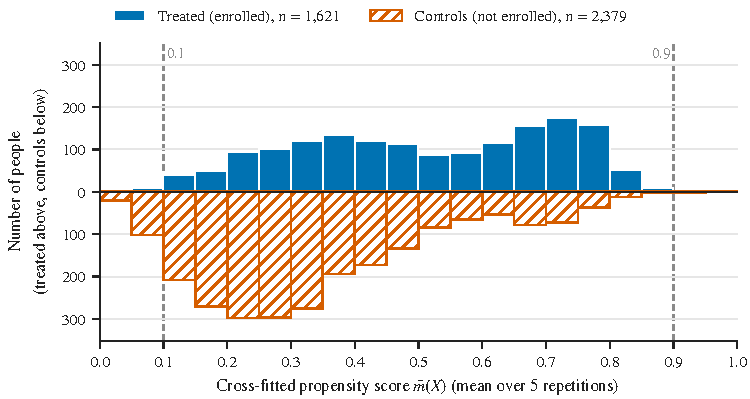
\includegraphics[width=0.75\textwidth]{figures/fig_propensity.pdf}
\caption{Overlap of the cross-fitted propensity score. Bars count people per bin of width
0.05 of $\bar m(X)$, the out-of-fold propensity from the primary specification (L2-penalized
logit on $B(X)$, 5 folds $\times$ 5 repetitions), averaged over repetitions and unclipped.
Enrolees ($\PrimaryNTreated$) are counted above the axis (solid bars) and non-enrolees
($\PrimaryNControl$) below it (hatched bars). The dashed lines at 0.1 and 0.9 mark the
trimming bounds of the trimmed-overlap check and the threshold of overlap rule O1. No
enrolee lies above 0.9. A share $\OverlapShareOutside$ of all people lies outside
$[0.1, 0.9]$, almost all of them non-enrolees below 0.1 (Table~\ref{tab:balance}). The
figure shows counts, so it has no error bars. The scores were computed outcome-blind, before
the design gate.}
\label{fig:propensity}
\end{figure}

\section{Results}
\label{sec:results}

Table~\ref{tab:main} reports the primary estimate in its first row. The cross-fitted AIPW
estimate of the ATT of enrolment on 1978 earnings is $\PrimaryEffect$ dollars (standard
error $\PrimarySE$), with 95\% confidence interval \ci{\PrimaryCILow}{\PrimaryCIHigh}.
Enrolees' mean 1978 earnings are $\PrimaryTreatedMean$ dollars and their estimated
counterfactual mean is $\PrimaryCFMean$, so the estimate is $\PrimaryRelEffect$\% of the
counterfactual mean, with a delta-method 95\% interval from $\PrimaryRelCILow$\% to
$\PrimaryRelCIHigh$\%. That relative interval is computed, as the plan specifies, from the
influence function averaged over repetitions; it omits the between-repetition variance term
in the primary standard error and is therefore slightly narrower than the dollar interval
divided by the counterfactual mean.

\emph{H1.} A zero ATT is not rejected ($p = \PrimaryP$). Read as an interval, the data are
compatible with effects from a loss of about $\absval{\PrimaryCILow}$ dollars to a gain of
about $\PrimaryCIHigh$ dollars in 1978, and they rule out effects outside that range at the
95\% level under the identifying assumption.

\emph{H1b.} Under unconfoundedness given the eleven covariates, the 90\% interval
\ci{\PrimaryCINinetyLow}{\PrimaryCINinetyHigh} lies inside $(-M, M) =
(-\EquivMargin, \EquivMargin)$, and the equivalence test gives $p = \PrimaryTOSTP$. The
smallest symmetric margin the interval would satisfy is $\PrimaryMinMargin$ dollars, and the
point estimate is $\PrimaryEffectOverMargin$ times $M$. Overlap rules O1 and O2 passed in
the same run, so the plan's additional condition on the trimmed-overlap interval did not
apply. This equivalence conclusion is conditional, and the condition is fragile: it is not
robust to an unobserved confounder as strong as the 1975-earnings covariates, which would move
the estimate by up to $\SensBenchEarnSeventyFiveBias$ dollars, so the result could be
produced by unobserved selection of that strength, and an unobserved 1976 earnings shock is
plausibly at least that strongly related to enrolment. The equivalence conclusion is also not
robust to a confounder as strong as the 1974-earnings covariates
(Section~\ref{sec:sensitivity}).

\emph{Selection on the 1975 shock (descriptive).} Panel~B of Table~\ref{tab:main} gives the
plan's fixed description. Given 1974 earnings and fixed characteristics, enrolees' 1975
earnings were $\absval{\SelectEarnPriorEffect}$ dollars lower than comparable non-enrolees'
(95\% interval \ci{\SelectEarnPriorCILow}{\SelectEarnPriorCIHigh}), about
$\absval{\SelectEarnPriorOverMargin}$ times $M$; this measures selection on the 1975 shock
and is not a test of the identifying assumption, which conditions on 1975 earnings. It is
reported to show the size of the selection the primary estimate must absorb, not as support
for that estimate.

\begin{table}[tbp]
\centering
\caption{ATT of enrolment on 1978 earnings: the primary estimate and every planned
robustness estimate (panel A, the same rows as Figure~\ref{fig:forest}), and a descriptive
measure of pre-program selection (panel B). The primary estimator is cross-fitted AIPW for
the ATT, with gradient-boosted outcome and L2-logit propensity models, 5 folds $\times$ 5
repetitions, and influence-function standard errors. $p$ is the two-sided $p$-value for
ATT $= 0$ (H1). $p_{\mathrm{TOST}}$ is the equivalence $p$-value for $|$ATT$| < M$ (H1b); it
is below 0.05 exactly when the 90\% CI lies within $\pm M$. ``Rejects 0'' and ``Within
$\pm M$'' are each run's own H1 and H1b decisions. ``--'' means the run did not compute the
quantity: the OLS row has no 90\% CI, TOST or equivalence decision, and the Hajek IPW row has
no $p$-values; its decisions come from its bootstrap-SE intervals. The H1b decisions hold
under unconfoundedness given the eleven covariates and are not robust to a confounder as
strong as earnings75 (Table~\ref{tab:sensitivity}). $^{a}$~A different estimand: the ATT
among the $\TrimN$ people ($\TrimNTreated$ enrolees) with $\bar m \in [0.1, 0.9]$.
$^{b}$~Set (a) conditions on age, educ, married, re74, re75, unemp74 and unemp75. Set (b)
conditions on all eleven covariates except re74 and unemp74. $^{c}$~A different estimand
and assumption: the ATT on re78 $-$ re74 under conditional parallel trends from 1974 to 1978,
given the time-invariant covariates. Its bias is upward if enrolees' 1974 earnings were
already transitorily depressed and downward if they were on a permanently lower growth path;
its sign is not known. $^{d}$~The same estimator with re75 as the outcome, conditioning on the
1974 covariates. The documented pre-program dip makes this nonzero whether or not the
identifying assumption holds, so it is neither a test of the assumption nor support for the
primary result, and no $p$-value is reported.}
\label{tab:main}
\footnotesize
\setlength{\tabcolsep}{3pt}
\resizebox{\textwidth}{!}{% Generated by code/tab_main.py from logged runs. Do not edit by hand; rerun the script.
% Needs \usepackage{booktabs,icomma} and % Generated by `crew.py numbers` from claims.jsonl. Do not edit by hand.
% Each macro is a number taken from a logged run; see claims.jsonl.
\newcommand{\PrimaryEffect}{-10}  % primary-effect
\newcommand{\PrimaryCILow}{-358}  % primary-ci-low
\newcommand{\PrimaryCIHigh}{338}  % primary-ci-high
\newcommand{\PrimarySE}{178}  % primary-se
\newcommand{\PrimaryP}{0.956}  % primary-p
\newcommand{\PrimaryCINinetyLow}{-302}  % primary-ci90-low
\newcommand{\PrimaryCINinetyHigh}{282}  % primary-ci90-high
\newcommand{\PrimaryTOSTP}{0.004}  % primary-tost-p
\newcommand{\PrimaryMinMargin}{302}  % primary-min-margin
\newcommand{\EquivMargin}{483.47}  % equiv-margin
\newcommand{\PrimaryRelEffect}{-0.1}  % primary-rel-effect
\newcommand{\PrimaryRelCILow}{-4.3}  % primary-rel-ci-low
\newcommand{\PrimaryRelCIHigh}{4.1}  % primary-rel-ci-high
\newcommand{\PrimaryCFMean}{7,940}  % primary-cf-mean
\newcommand{\PrimaryTreatedMean}{7,930}  % primary-treated-mean
\newcommand{\PrimaryEffectOverMargin}{-0.02}  % primary-effect-over-margin
\newcommand{\PrimaryN}{4,000}  % primary-n
\newcommand{\PrimaryNTreated}{1,621}  % primary-n-treated
\newcommand{\PrimaryNControl}{2,379}  % primary-n-control
\newcommand{\PrimaryNClipped}{0}  % primary-n-clipped
\newcommand{\OverlapShareOutside}{0.033}  % overlap-share-outside
\newcommand{\OverlapTreatedAboveNineTenths}{0.000}  % overlap-treated-above-09
\newcommand{\SecEarnNextEffect}{-112}  % sec-re79-effect
\newcommand{\SecEarnNextSE}{196}  % sec-re79-se
\newcommand{\SecEarnNextCILow}{-495}  % sec-re79-ci-low
\newcommand{\SecEarnNextCIHigh}{272}  % sec-re79-ci-high
\newcommand{\SecEarnNextP}{0.568}  % sec-re79-p
\newcommand{\SecEarnNextPRW}{0.744}  % sec-re79-p-rw
\newcommand{\SecEarnNextMaxTLow}{-596}  % sec-re79-maxt-low
\newcommand{\SecEarnNextMaxTHigh}{373}  % sec-re79-maxt-high
\newcommand{\SecEmployedEffect}{1.0}  % sec-employed78-effect
\newcommand{\SecEmployedSE}{1.4}  % sec-employed78-se
\newcommand{\SecEmployedCILow}{-1.7}  % sec-employed78-ci-low
\newcommand{\SecEmployedCIHigh}{3.7}  % sec-employed78-ci-high
\newcommand{\SecEmployedP}{0.465}  % sec-employed78-p
\newcommand{\SecEmployedPRW}{0.744}  % sec-employed78-p-rw
\newcommand{\SecEmployedMaxTLow}{-2.4}  % sec-employed78-maxt-low
\newcommand{\SecEmployedMaxTHigh}{4.4}  % sec-employed78-maxt-high
\newcommand{\SecHoursEffect}{48.2}  % sec-hours78-effect
\newcommand{\SecHoursSE}{26.3}  % sec-hours78-se
\newcommand{\SecHoursCILow}{-3.4}  % sec-hours78-ci-low
\newcommand{\SecHoursCIHigh}{99.8}  % sec-hours78-ci-high
\newcommand{\SecHoursP}{0.067}  % sec-hours78-p
\newcommand{\SecHoursPRW}{0.204}  % sec-hours78-p-rw
\newcommand{\SecHoursMaxTLow}{-17.0}  % sec-hours78-maxt-low
\newcommand{\SecHoursMaxTHigh}{113.5}  % sec-hours78-maxt-high
\newcommand{\SecBenefitsEffect}{87}  % sec-benefits78-effect
\newcommand{\SecBenefitsSE}{43}  % sec-benefits78-se
\newcommand{\SecBenefitsCILow}{3}  % sec-benefits78-ci-low
\newcommand{\SecBenefitsCIHigh}{171}  % sec-benefits78-ci-high
\newcommand{\SecBenefitsP}{0.044}  % sec-benefits78-p
\newcommand{\SecBenefitsPRW}{0.166}  % sec-benefits78-p-rw
\newcommand{\SecBenefitsMaxTLow}{-20}  % sec-benefits78-maxt-low
\newcommand{\SecBenefitsMaxTHigh}{194}  % sec-benefits78-maxt-high
\newcommand{\SecWellbeingEffect}{0.06}  % sec-wellbeing78-effect
\newcommand{\SecWellbeingSE}{0.07}  % sec-wellbeing78-se
\newcommand{\SecWellbeingCILow}{-0.08}  % sec-wellbeing78-ci-low
\newcommand{\SecWellbeingCIHigh}{0.21}  % sec-wellbeing78-ci-high
\newcommand{\SecWellbeingP}{0.383}  % sec-wellbeing78-p
\newcommand{\SecWellbeingPRW}{0.744}  % sec-wellbeing78-p-rw
\newcommand{\SecWellbeingMaxTLow}{-0.12}  % sec-wellbeing78-maxt-low
\newcommand{\SecWellbeingMaxTHigh}{0.24}  % sec-wellbeing78-maxt-high
\newcommand{\SecMaxTCrit}{2.477}  % sec-maxt-crit
\newcommand{\SecNDetected}{0}  % sec-n-detected
\newcommand{\SecWellbeingEffectSD}{0.036}  % sec-wellbeing78-effect-sd
\newcommand{\SecWellbeingControlSD}{1.78}  % sec-wellbeing78-control-sd
\newcommand{\SelectEarnPriorEffect}{-3,541}  % select-re75-effect
\newcommand{\SelectEarnPriorCILow}{-3,878}  % select-re75-ci-low
\newcommand{\SelectEarnPriorCIHigh}{-3,204}  % select-re75-ci-high
\newcommand{\SelectEarnPriorOverMargin}{-7.3}  % select-re75-over-margin
\newcommand{\TrimEffect}{36}  % trim-effect
\newcommand{\TrimCILow}{-300}  % trim-ci-low
\newcommand{\TrimCIHigh}{371}  % trim-ci-high
\newcommand{\TrimN}{3,867}  % trim-n
\newcommand{\TrimCINinetyLow}{-246}  % trim-ci90-low
\newcommand{\TrimCINinetyHigh}{317}  % trim-ci90-high
\newcommand{\CovsetAEffect}{-32}  % covset-a-effect
\newcommand{\CovsetACILow}{-370}  % covset-a-ci-low
\newcommand{\CovsetACIHigh}{307}  % covset-a-ci-high
\newcommand{\CovsetAN}{4,000}  % covset-a-n
\newcommand{\CovsetACINinetyLow}{-316}  % covset-a-ci90-low
\newcommand{\CovsetACINinetyHigh}{253}  % covset-a-ci90-high
\newcommand{\CovsetBEffect}{-139}  % covset-b-effect
\newcommand{\CovsetBCILow}{-494}  % covset-b-ci-low
\newcommand{\CovsetBCIHigh}{215}  % covset-b-ci-high
\newcommand{\CovsetBN}{4,000}  % covset-b-n
\newcommand{\CovsetBCINinetyLow}{-437}  % covset-b-ci90-low
\newcommand{\CovsetBCINinetyHigh}{158}  % covset-b-ci90-high
\newcommand{\LearnerLinearEffect}{-116}  % learner-linear-effect
\newcommand{\LearnerLinearCILow}{-450}  % learner-linear-ci-low
\newcommand{\LearnerLinearCIHigh}{218}  % learner-linear-ci-high
\newcommand{\LearnerLinearN}{4,000}  % learner-linear-n
\newcommand{\LearnerLinearCINinetyLow}{-396}  % learner-linear-ci90-low
\newcommand{\LearnerLinearCINinetyHigh}{165}  % learner-linear-ci90-high
\newcommand{\LearnerRFEffect}{-10}  % learner-rf-effect
\newcommand{\LearnerRFCILow}{-358}  % learner-rf-ci-low
\newcommand{\LearnerRFCIHigh}{338}  % learner-rf-ci-high
\newcommand{\LearnerRFN}{4,000}  % learner-rf-n
\newcommand{\LearnerRFCINinetyLow}{-302}  % learner-rf-ci90-low
\newcommand{\LearnerRFCINinetyHigh}{282}  % learner-rf-ci90-high
\newcommand{\DiffSeventyFourEffect}{-1,087}  % diff74-effect
\newcommand{\DiffSeventyFourCILow}{-1,496}  % diff74-ci-low
\newcommand{\DiffSeventyFourCIHigh}{-678}  % diff74-ci-high
\newcommand{\DiffSeventyFourN}{4,000}  % diff74-n
\newcommand{\DiffSeventyFourCINinetyLow}{-1,430}  % diff74-ci90-low
\newcommand{\DiffSeventyFourCINinetyHigh}{-743}  % diff74-ci90-high
\newcommand{\OLSEffect}{-127}  % ols-effect
\newcommand{\OLSCILow}{-434}  % ols-ci-low
\newcommand{\OLSCIHigh}{181}  % ols-ci-high
\newcommand{\OLSN}{4,000}  % ols-n
\newcommand{\IPWEffect}{-191}  % ipw-effect
\newcommand{\IPWCILow}{-521}  % ipw-ci-low
\newcommand{\IPWCIHigh}{139}  % ipw-ci-high
\newcommand{\IPWN}{4,000}  % ipw-n
\newcommand{\IPWCINinetyLow}{-468}  % ipw-ci90-low
\newcommand{\IPWCINinetyHigh}{86}  % ipw-ci90-high
\newcommand{\TrimNTreated}{1,611}  % trim-n-treated
\newcommand{\TrimNDropped}{133}  % trim-n-dropped
\newcommand{\SensRsqMargin}{0.060}  % sens-r2-margin
\newcommand{\SensTargetMargin}{483}  % sens-target-margin
\newcommand{\SensRsqZero}{0.042}  % sens-r2-zero
\newcommand{\SensTargetZero}{338}  % sens-target-zero
\newcommand{\SensRsqEquiv}{0.023}  % sens-r2-equiv
\newcommand{\SensTargetEquiv}{181}  % sens-target-equiv
\newcommand{\SensBenchAgeRsqD}{0.010}  % sens-bench-age-r2d
\newcommand{\SensBenchAgeRsqY}{0.025}  % sens-bench-age-r2y
\newcommand{\SensBenchAgeBias}{128}  % sens-bench-age-bias
\newcommand{\SensBenchEducRsqD}{0.024}  % sens-bench-educ-r2d
\newcommand{\SensBenchEducRsqY}{0.010}  % sens-bench-educ-r2y
\newcommand{\SensBenchEducBias}{126}  % sens-bench-educ-bias
\newcommand{\SensBenchMarriedRsqD}{0.000}  % sens-bench-married-r2d
\newcommand{\SensBenchMarriedRsqY}{0.001}  % sens-bench-married-r2y
\newcommand{\SensBenchMarriedBias}{6}  % sens-bench-married-bias
\newcommand{\SensBenchUrbanRsqD}{0.000}  % sens-bench-urban-r2d
\newcommand{\SensBenchUrbanRsqY}{0.001}  % sens-bench-urban-r2y
\newcommand{\SensBenchUrbanBias}{5}  % sens-bench-urban-bias
\newcommand{\SensBenchRegionRsqD}{0.000}  % sens-bench-region-r2d
\newcommand{\SensBenchRegionRsqY}{0.000}  % sens-bench-region-r2y
\newcommand{\SensBenchRegionBias}{0}  % sens-bench-region-bias
\newcommand{\SensBenchChildrenRsqD}{0.000}  % sens-bench-children-r2d
\newcommand{\SensBenchChildrenRsqY}{0.000}  % sens-bench-children-r2y
\newcommand{\SensBenchChildrenBias}{1}  % sens-bench-children-bias
\newcommand{\SensBenchHealthRsqD}{0.002}  % sens-bench-health-r2d
\newcommand{\SensBenchHealthRsqY}{0.000}  % sens-bench-health-r2y
\newcommand{\SensBenchHealthBias}{6}  % sens-bench-health-bias
\newcommand{\SensBenchEarnSeventyFourRsqD}{0.010}  % sens-bench-earn74-r2d
\newcommand{\SensBenchEarnSeventyFourRsqY}{0.066}  % sens-bench-earn74-r2y
\newcommand{\SensBenchEarnSeventyFourBias}{204}  % sens-bench-earn74-bias
\newcommand{\SensBenchEarnSeventyFiveRsqD}{0.189}  % sens-bench-earn75-r2d
\newcommand{\SensBenchEarnSeventyFiveRsqY}{0.237}  % sens-bench-earn75-r2y
\newcommand{\SensBenchEarnSeventyFiveBias}{1,716}  % sens-bench-earn75-bias
\newcommand{\SensTauZero}{-127}  % sens-tau00
\newcommand{\SensSigmaZero}{4,407}  % sens-sigma-zero
\newcommand{\MissingEarnTreated}{0}  % missing-re78-treated
\newcommand{\InvalidEarnTreated}{0}  % invalid-re78-treated
\newcommand{\MissingEarnControl}{0}  % missing-re78-control
\newcommand{\InvalidEarnControl}{0}  % invalid-re78-control
\newcommand{\MissingEarnNextTreated}{0}  % missing-re79-treated
\newcommand{\InvalidEarnNextTreated}{0}  % invalid-re79-treated
\newcommand{\MissingEarnNextControl}{0}  % missing-re79-control
\newcommand{\InvalidEarnNextControl}{0}  % invalid-re79-control
\newcommand{\MissingEmployedTreated}{0}  % missing-employed78-treated
\newcommand{\InvalidEmployedTreated}{0}  % invalid-employed78-treated
\newcommand{\MissingEmployedControl}{0}  % missing-employed78-control
\newcommand{\InvalidEmployedControl}{0}  % invalid-employed78-control
\newcommand{\MissingHoursTreated}{0}  % missing-hours78-treated
\newcommand{\InvalidHoursTreated}{0}  % invalid-hours78-treated
\newcommand{\MissingHoursControl}{0}  % missing-hours78-control
\newcommand{\InvalidHoursControl}{0}  % invalid-hours78-control
\newcommand{\MissingBenefitsTreated}{0}  % missing-benefits78-treated
\newcommand{\InvalidBenefitsTreated}{0}  % invalid-benefits78-treated
\newcommand{\MissingBenefitsControl}{0}  % missing-benefits78-control
\newcommand{\InvalidBenefitsControl}{0}  % invalid-benefits78-control
\newcommand{\MissingWellbeingTreated}{0}  % missing-wellbeing78-treated
\newcommand{\InvalidWellbeingTreated}{0}  % invalid-wellbeing78-treated
\newcommand{\MissingWellbeingControl}{0}  % missing-wellbeing78-control
\newcommand{\InvalidWellbeingControl}{0}  % invalid-wellbeing78-control
 for the macros
% (icomma keeps the thousands comma in math mode, e.g. $1,716$, without a space).
\begin{tabular}{@{}l r r c c r r c c r@{}}
\toprule
Specification & Estimate & SE & 95\% CI & 90\% CI & $p$ & $p_{\mathrm{TOST}}$ & Rejects 0 & Within $\pm M$ & $n$ \\
\midrule
\multicolumn{10}{@{}l}{\emph{A. ATT of enrolment on 1978 earnings (nominal dollars)}} \\
Primary: cross-fitted AIPW & $\PrimaryEffect$ & $\PrimarySE$ & [$\PrimaryCILow$, $\PrimaryCIHigh$] & [$\PrimaryCINinetyLow$, $\PrimaryCINinetyHigh$] & $\PrimaryP$ & $\PrimaryTOSTP$ & no & yes & $\PrimaryN$ \\
Trimmed overlap, $\bar m \in [0.1, 0.9]$$^{a}$ & $\TrimEffect$ & $171$ & [$\TrimCILow$, $\TrimCIHigh$] & [$\TrimCINinetyLow$, $\TrimCINinetyHigh$] & $0.835$ & $0.004$ & no & yes & $\TrimN$ \\
Covariate set (a)$^{b}$ & $\CovsetAEffect$ & $173$ & [$\CovsetACILow$, $\CovsetACIHigh$] & [$\CovsetACINinetyLow$, $\CovsetACINinetyHigh$] & $0.855$ & $0.004$ & no & yes & $\CovsetAN$ \\
Covariate set (b)$^{b}$ & $\CovsetBEffect$ & $181$ & [$\CovsetBCILow$, $\CovsetBCIHigh$] & [$\CovsetBCINinetyLow$, $\CovsetBCINinetyHigh$] & $0.441$ & $0.029$ & no & yes & $\CovsetBN$ \\
Parametric nuisances & $\LearnerLinearEffect$ & $170$ & [$\LearnerLinearCILow$, $\LearnerLinearCIHigh$] & [$\LearnerLinearCINinetyLow$, $\LearnerLinearCINinetyHigh$] & $0.497$ & $0.015$ & no & yes & $\LearnerLinearN$ \\
Random-forest nuisances & $\LearnerRFEffect$ & $178$ & [$\LearnerRFCILow$, $\LearnerRFCIHigh$] & [$\LearnerRFCINinetyLow$, $\LearnerRFCINinetyHigh$] & $0.955$ & $0.004$ & no & yes & $\LearnerRFN$ \\
OLS coefficient (HC2) & $\OLSEffect$ & $157$ & [$\OLSCILow$, $\OLSCIHigh$] & -- & $0.420$ & -- & no & -- & $\OLSN$ \\
Hajek IPW (bootstrap SE) & $\IPWEffect$ & $168$ & [$\IPWCILow$, $\IPWCIHigh$] & [$\IPWCINinetyLow$, $\IPWCINinetyHigh$] & -- & -- & no & yes & $\IPWN$ \\
Conditional DiD, re78 $-$ re74$^{c}$ & $\DiffSeventyFourEffect$ & $209$ & [$\DiffSeventyFourCILow$, $\DiffSeventyFourCIHigh$] & [$\DiffSeventyFourCINinetyLow$, $\DiffSeventyFourCINinetyHigh$] & $<0.001$ & $0.998$ & yes & no & $\DiffSeventyFourN$ \\
\midrule
\multicolumn{10}{@{}l}{\emph{B. Descriptive, not an estimate of the ATT: selection on the 1975 earnings shock$^{d}$}} \\
re75 given 1974 covariates & $\SelectEarnPriorEffect$ & $172$ & [$\SelectEarnPriorCILow$, $\SelectEarnPriorCIHigh$] & -- & -- & -- & -- & -- & $4,000$ \\
\midrule
\multicolumn{10}{@{}l}{Equivalence margin $M = \$\EquivMargin$ (10\% of participants' mean 1975 earnings, fixed before any outcome was read).} \\
\bottomrule
\end{tabular}
}
\end{table}

\section{Secondary outcomes}
\label{sec:secondary}

Table~\ref{tab:secondary} reports the five secondary outcomes. None is detected:
$\SecNDetected$ of five has a Romano--Wolf adjusted $p$ below 0.05. For 1979 earnings the
estimate is $\SecEarnNextEffect$ dollars, with simultaneous interval
\ci{\SecEarnNextMaxTLow}{\SecEarnNextMaxTHigh} (Romano--Wolf $p = \SecEarnNextPRW$). For
employment in 1978 it is $\SecEmployedEffect$ percentage points
\ci{\SecEmployedMaxTLow}{\SecEmployedMaxTHigh}; for hours, $\SecHoursEffect$ hours
\ci{\SecHoursMaxTLow}{\SecHoursMaxTHigh}; for the well-being score, $\SecWellbeingEffect$
scale points \ci{\SecWellbeingMaxTLow}{\SecWellbeingMaxTHigh}, which is $\SecWellbeingEffectSD$
standard deviations of the non-enrolee distribution
\ci{\SecWellbeingMaxTLowSD}{\SecWellbeingMaxTHighSD}. For benefits received the estimate is
$\SecBenefitsEffect$ dollars \ci{\SecBenefitsMaxTLow}{\SecBenefitsMaxTHigh}. Its unadjusted
$p$ is $\SecBenefitsP$, but its Romano--Wolf $p$ is $\SecBenefitsPRW$, so under the
pre-specified rule it is not detected and is not reported as an effect of enrolment; its
simultaneous interval includes zero.

The bootstrap behind the Romano--Wolf $p$-values and the max-$t$ intervals uses, as the plan
specifies, the influence function averaged over repetitions, while the standard errors
include the between-repetition spread. The adjusted $p$-values and simultaneous intervals are
therefore slightly anti-conservative relative to the standard-error column. No detection
decision depends on this: the smallest Romano--Wolf $p$ is $\SecBenefitsPRW$.

\begin{table}[tbp]
\centering
\caption{Secondary outcome family (H2). Each outcome is estimated with the primary estimator
on the same folds and propensity fits, with $n = \PrimaryN$ and no missing or inadmissible
values. Romano--Wolf step-down $p$-values and single-step max-$t$ simultaneous 95\% intervals
come from one Gaussian multiplier bootstrap on the influence functions, with the nuisance
models not re-fitted. An outcome counts as ``detected'' if and only if its Romano--Wolf
$p < 0.05$; none is. Unadjusted $p$-values are shown for reference only, and an outcome with
an unadjusted $p$ below 0.05 but a Romano--Wolf $p$ above it (benefits78) is not described as
affected. Per-outcome unadjusted intervals are not reported. The bootstrap uses the influence
function averaged over repetitions, so its scale omits the between-repetition variance in the
standard errors; the Romano--Wolf $p$-values and max-$t$ intervals are slightly
anti-conservative relative to the SE column. $^{a}$~An integer scale assumed to be
$[0, 10]$; the brief documents no scale. $^{b}$~In units of the SD of wellbeing78 among
non-enrolees ($\SecWellbeingControlSD$ scale points).}
\label{tab:secondary}
\footnotesize
\setlength{\tabcolsep}{4pt}
\resizebox{\textwidth}{!}{% Generated by code/tab_secondary.py from logged runs. Do not edit by hand; rerun the script.
% Needs \usepackage{booktabs,icomma} and % Generated by `crew.py numbers` from claims.jsonl. Do not edit by hand.
% Each macro is a number taken from a logged run; see claims.jsonl.
\newcommand{\PrimaryEffect}{-10}  % primary-effect
\newcommand{\PrimaryCILow}{-358}  % primary-ci-low
\newcommand{\PrimaryCIHigh}{338}  % primary-ci-high
\newcommand{\PrimarySE}{178}  % primary-se
\newcommand{\PrimaryP}{0.956}  % primary-p
\newcommand{\PrimaryCINinetyLow}{-302}  % primary-ci90-low
\newcommand{\PrimaryCINinetyHigh}{282}  % primary-ci90-high
\newcommand{\PrimaryTOSTP}{0.004}  % primary-tost-p
\newcommand{\PrimaryMinMargin}{302}  % primary-min-margin
\newcommand{\EquivMargin}{483.47}  % equiv-margin
\newcommand{\PrimaryRelEffect}{-0.1}  % primary-rel-effect
\newcommand{\PrimaryRelCILow}{-4.3}  % primary-rel-ci-low
\newcommand{\PrimaryRelCIHigh}{4.1}  % primary-rel-ci-high
\newcommand{\PrimaryCFMean}{7,940}  % primary-cf-mean
\newcommand{\PrimaryTreatedMean}{7,930}  % primary-treated-mean
\newcommand{\PrimaryEffectOverMargin}{-0.02}  % primary-effect-over-margin
\newcommand{\PrimaryN}{4,000}  % primary-n
\newcommand{\PrimaryNTreated}{1,621}  % primary-n-treated
\newcommand{\PrimaryNControl}{2,379}  % primary-n-control
\newcommand{\PrimaryNClipped}{0}  % primary-n-clipped
\newcommand{\OverlapShareOutside}{0.033}  % overlap-share-outside
\newcommand{\OverlapTreatedAboveNineTenths}{0.000}  % overlap-treated-above-09
\newcommand{\SecEarnNextEffect}{-112}  % sec-re79-effect
\newcommand{\SecEarnNextSE}{196}  % sec-re79-se
\newcommand{\SecEarnNextCILow}{-495}  % sec-re79-ci-low
\newcommand{\SecEarnNextCIHigh}{272}  % sec-re79-ci-high
\newcommand{\SecEarnNextP}{0.568}  % sec-re79-p
\newcommand{\SecEarnNextPRW}{0.744}  % sec-re79-p-rw
\newcommand{\SecEarnNextMaxTLow}{-596}  % sec-re79-maxt-low
\newcommand{\SecEarnNextMaxTHigh}{373}  % sec-re79-maxt-high
\newcommand{\SecEmployedEffect}{1.0}  % sec-employed78-effect
\newcommand{\SecEmployedSE}{1.4}  % sec-employed78-se
\newcommand{\SecEmployedCILow}{-1.7}  % sec-employed78-ci-low
\newcommand{\SecEmployedCIHigh}{3.7}  % sec-employed78-ci-high
\newcommand{\SecEmployedP}{0.465}  % sec-employed78-p
\newcommand{\SecEmployedPRW}{0.744}  % sec-employed78-p-rw
\newcommand{\SecEmployedMaxTLow}{-2.4}  % sec-employed78-maxt-low
\newcommand{\SecEmployedMaxTHigh}{4.4}  % sec-employed78-maxt-high
\newcommand{\SecHoursEffect}{48.2}  % sec-hours78-effect
\newcommand{\SecHoursSE}{26.3}  % sec-hours78-se
\newcommand{\SecHoursCILow}{-3.4}  % sec-hours78-ci-low
\newcommand{\SecHoursCIHigh}{99.8}  % sec-hours78-ci-high
\newcommand{\SecHoursP}{0.067}  % sec-hours78-p
\newcommand{\SecHoursPRW}{0.204}  % sec-hours78-p-rw
\newcommand{\SecHoursMaxTLow}{-17.0}  % sec-hours78-maxt-low
\newcommand{\SecHoursMaxTHigh}{113.5}  % sec-hours78-maxt-high
\newcommand{\SecBenefitsEffect}{87}  % sec-benefits78-effect
\newcommand{\SecBenefitsSE}{43}  % sec-benefits78-se
\newcommand{\SecBenefitsCILow}{3}  % sec-benefits78-ci-low
\newcommand{\SecBenefitsCIHigh}{171}  % sec-benefits78-ci-high
\newcommand{\SecBenefitsP}{0.044}  % sec-benefits78-p
\newcommand{\SecBenefitsPRW}{0.166}  % sec-benefits78-p-rw
\newcommand{\SecBenefitsMaxTLow}{-20}  % sec-benefits78-maxt-low
\newcommand{\SecBenefitsMaxTHigh}{194}  % sec-benefits78-maxt-high
\newcommand{\SecWellbeingEffect}{0.06}  % sec-wellbeing78-effect
\newcommand{\SecWellbeingSE}{0.07}  % sec-wellbeing78-se
\newcommand{\SecWellbeingCILow}{-0.08}  % sec-wellbeing78-ci-low
\newcommand{\SecWellbeingCIHigh}{0.21}  % sec-wellbeing78-ci-high
\newcommand{\SecWellbeingP}{0.383}  % sec-wellbeing78-p
\newcommand{\SecWellbeingPRW}{0.744}  % sec-wellbeing78-p-rw
\newcommand{\SecWellbeingMaxTLow}{-0.12}  % sec-wellbeing78-maxt-low
\newcommand{\SecWellbeingMaxTHigh}{0.24}  % sec-wellbeing78-maxt-high
\newcommand{\SecMaxTCrit}{2.477}  % sec-maxt-crit
\newcommand{\SecNDetected}{0}  % sec-n-detected
\newcommand{\SecWellbeingEffectSD}{0.036}  % sec-wellbeing78-effect-sd
\newcommand{\SecWellbeingControlSD}{1.78}  % sec-wellbeing78-control-sd
\newcommand{\SelectEarnPriorEffect}{-3,541}  % select-re75-effect
\newcommand{\SelectEarnPriorCILow}{-3,878}  % select-re75-ci-low
\newcommand{\SelectEarnPriorCIHigh}{-3,204}  % select-re75-ci-high
\newcommand{\SelectEarnPriorOverMargin}{-7.3}  % select-re75-over-margin
\newcommand{\TrimEffect}{36}  % trim-effect
\newcommand{\TrimCILow}{-300}  % trim-ci-low
\newcommand{\TrimCIHigh}{371}  % trim-ci-high
\newcommand{\TrimN}{3,867}  % trim-n
\newcommand{\TrimCINinetyLow}{-246}  % trim-ci90-low
\newcommand{\TrimCINinetyHigh}{317}  % trim-ci90-high
\newcommand{\CovsetAEffect}{-32}  % covset-a-effect
\newcommand{\CovsetACILow}{-370}  % covset-a-ci-low
\newcommand{\CovsetACIHigh}{307}  % covset-a-ci-high
\newcommand{\CovsetAN}{4,000}  % covset-a-n
\newcommand{\CovsetACINinetyLow}{-316}  % covset-a-ci90-low
\newcommand{\CovsetACINinetyHigh}{253}  % covset-a-ci90-high
\newcommand{\CovsetBEffect}{-139}  % covset-b-effect
\newcommand{\CovsetBCILow}{-494}  % covset-b-ci-low
\newcommand{\CovsetBCIHigh}{215}  % covset-b-ci-high
\newcommand{\CovsetBN}{4,000}  % covset-b-n
\newcommand{\CovsetBCINinetyLow}{-437}  % covset-b-ci90-low
\newcommand{\CovsetBCINinetyHigh}{158}  % covset-b-ci90-high
\newcommand{\LearnerLinearEffect}{-116}  % learner-linear-effect
\newcommand{\LearnerLinearCILow}{-450}  % learner-linear-ci-low
\newcommand{\LearnerLinearCIHigh}{218}  % learner-linear-ci-high
\newcommand{\LearnerLinearN}{4,000}  % learner-linear-n
\newcommand{\LearnerLinearCINinetyLow}{-396}  % learner-linear-ci90-low
\newcommand{\LearnerLinearCINinetyHigh}{165}  % learner-linear-ci90-high
\newcommand{\LearnerRFEffect}{-10}  % learner-rf-effect
\newcommand{\LearnerRFCILow}{-358}  % learner-rf-ci-low
\newcommand{\LearnerRFCIHigh}{338}  % learner-rf-ci-high
\newcommand{\LearnerRFN}{4,000}  % learner-rf-n
\newcommand{\LearnerRFCINinetyLow}{-302}  % learner-rf-ci90-low
\newcommand{\LearnerRFCINinetyHigh}{282}  % learner-rf-ci90-high
\newcommand{\DiffSeventyFourEffect}{-1,087}  % diff74-effect
\newcommand{\DiffSeventyFourCILow}{-1,496}  % diff74-ci-low
\newcommand{\DiffSeventyFourCIHigh}{-678}  % diff74-ci-high
\newcommand{\DiffSeventyFourN}{4,000}  % diff74-n
\newcommand{\DiffSeventyFourCINinetyLow}{-1,430}  % diff74-ci90-low
\newcommand{\DiffSeventyFourCINinetyHigh}{-743}  % diff74-ci90-high
\newcommand{\OLSEffect}{-127}  % ols-effect
\newcommand{\OLSCILow}{-434}  % ols-ci-low
\newcommand{\OLSCIHigh}{181}  % ols-ci-high
\newcommand{\OLSN}{4,000}  % ols-n
\newcommand{\IPWEffect}{-191}  % ipw-effect
\newcommand{\IPWCILow}{-521}  % ipw-ci-low
\newcommand{\IPWCIHigh}{139}  % ipw-ci-high
\newcommand{\IPWN}{4,000}  % ipw-n
\newcommand{\IPWCINinetyLow}{-468}  % ipw-ci90-low
\newcommand{\IPWCINinetyHigh}{86}  % ipw-ci90-high
\newcommand{\TrimNTreated}{1,611}  % trim-n-treated
\newcommand{\TrimNDropped}{133}  % trim-n-dropped
\newcommand{\SensRsqMargin}{0.060}  % sens-r2-margin
\newcommand{\SensTargetMargin}{483}  % sens-target-margin
\newcommand{\SensRsqZero}{0.042}  % sens-r2-zero
\newcommand{\SensTargetZero}{338}  % sens-target-zero
\newcommand{\SensRsqEquiv}{0.023}  % sens-r2-equiv
\newcommand{\SensTargetEquiv}{181}  % sens-target-equiv
\newcommand{\SensBenchAgeRsqD}{0.010}  % sens-bench-age-r2d
\newcommand{\SensBenchAgeRsqY}{0.025}  % sens-bench-age-r2y
\newcommand{\SensBenchAgeBias}{128}  % sens-bench-age-bias
\newcommand{\SensBenchEducRsqD}{0.024}  % sens-bench-educ-r2d
\newcommand{\SensBenchEducRsqY}{0.010}  % sens-bench-educ-r2y
\newcommand{\SensBenchEducBias}{126}  % sens-bench-educ-bias
\newcommand{\SensBenchMarriedRsqD}{0.000}  % sens-bench-married-r2d
\newcommand{\SensBenchMarriedRsqY}{0.001}  % sens-bench-married-r2y
\newcommand{\SensBenchMarriedBias}{6}  % sens-bench-married-bias
\newcommand{\SensBenchUrbanRsqD}{0.000}  % sens-bench-urban-r2d
\newcommand{\SensBenchUrbanRsqY}{0.001}  % sens-bench-urban-r2y
\newcommand{\SensBenchUrbanBias}{5}  % sens-bench-urban-bias
\newcommand{\SensBenchRegionRsqD}{0.000}  % sens-bench-region-r2d
\newcommand{\SensBenchRegionRsqY}{0.000}  % sens-bench-region-r2y
\newcommand{\SensBenchRegionBias}{0}  % sens-bench-region-bias
\newcommand{\SensBenchChildrenRsqD}{0.000}  % sens-bench-children-r2d
\newcommand{\SensBenchChildrenRsqY}{0.000}  % sens-bench-children-r2y
\newcommand{\SensBenchChildrenBias}{1}  % sens-bench-children-bias
\newcommand{\SensBenchHealthRsqD}{0.002}  % sens-bench-health-r2d
\newcommand{\SensBenchHealthRsqY}{0.000}  % sens-bench-health-r2y
\newcommand{\SensBenchHealthBias}{6}  % sens-bench-health-bias
\newcommand{\SensBenchEarnSeventyFourRsqD}{0.010}  % sens-bench-earn74-r2d
\newcommand{\SensBenchEarnSeventyFourRsqY}{0.066}  % sens-bench-earn74-r2y
\newcommand{\SensBenchEarnSeventyFourBias}{204}  % sens-bench-earn74-bias
\newcommand{\SensBenchEarnSeventyFiveRsqD}{0.189}  % sens-bench-earn75-r2d
\newcommand{\SensBenchEarnSeventyFiveRsqY}{0.237}  % sens-bench-earn75-r2y
\newcommand{\SensBenchEarnSeventyFiveBias}{1,716}  % sens-bench-earn75-bias
\newcommand{\SensTauZero}{-127}  % sens-tau00
\newcommand{\SensSigmaZero}{4,407}  % sens-sigma-zero
\newcommand{\MissingEarnTreated}{0}  % missing-re78-treated
\newcommand{\InvalidEarnTreated}{0}  % invalid-re78-treated
\newcommand{\MissingEarnControl}{0}  % missing-re78-control
\newcommand{\InvalidEarnControl}{0}  % invalid-re78-control
\newcommand{\MissingEarnNextTreated}{0}  % missing-re79-treated
\newcommand{\InvalidEarnNextTreated}{0}  % invalid-re79-treated
\newcommand{\MissingEarnNextControl}{0}  % missing-re79-control
\newcommand{\InvalidEarnNextControl}{0}  % invalid-re79-control
\newcommand{\MissingEmployedTreated}{0}  % missing-employed78-treated
\newcommand{\InvalidEmployedTreated}{0}  % invalid-employed78-treated
\newcommand{\MissingEmployedControl}{0}  % missing-employed78-control
\newcommand{\InvalidEmployedControl}{0}  % invalid-employed78-control
\newcommand{\MissingHoursTreated}{0}  % missing-hours78-treated
\newcommand{\InvalidHoursTreated}{0}  % invalid-hours78-treated
\newcommand{\MissingHoursControl}{0}  % missing-hours78-control
\newcommand{\InvalidHoursControl}{0}  % invalid-hours78-control
\newcommand{\MissingBenefitsTreated}{0}  % missing-benefits78-treated
\newcommand{\InvalidBenefitsTreated}{0}  % invalid-benefits78-treated
\newcommand{\MissingBenefitsControl}{0}  % missing-benefits78-control
\newcommand{\InvalidBenefitsControl}{0}  % invalid-benefits78-control
\newcommand{\MissingWellbeingTreated}{0}  % missing-wellbeing78-treated
\newcommand{\InvalidWellbeingTreated}{0}  % invalid-wellbeing78-treated
\newcommand{\MissingWellbeingControl}{0}  % missing-wellbeing78-control
\newcommand{\InvalidWellbeingControl}{0}  % invalid-wellbeing78-control
 for the macros
% (icomma keeps the thousands comma in math mode, e.g. $1,716$, without a space).
\begin{tabular}{@{}l r r r r c c@{}}
\toprule
Outcome (unit) & Estimate & SE & $p$, unadjusted & $p$, Romano--Wolf & Max-$t$ simultaneous 95\% interval & Detected \\
\midrule
re79 (nominal \$) & $\SecEarnNextEffect$ & $\SecEarnNextSE$ & $\SecEarnNextP$ & $\SecEarnNextPRW$ & [$\SecEarnNextMaxTLow$, $\SecEarnNextMaxTHigh$] & no \\
employed78 (percentage points) & $\SecEmployedEffect$ & $\SecEmployedSE$ & $\SecEmployedP$ & $\SecEmployedPRW$ & [$\SecEmployedMaxTLow$, $\SecEmployedMaxTHigh$] & no \\
hours78 (hours) & $\SecHoursEffect$ & $\SecHoursSE$ & $\SecHoursP$ & $\SecHoursPRW$ & [$\SecHoursMaxTLow$, $\SecHoursMaxTHigh$] & no \\
benefits78 (nominal \$) & $\SecBenefitsEffect$ & $\SecBenefitsSE$ & $\SecBenefitsP$ & $\SecBenefitsPRW$ & [$\SecBenefitsMaxTLow$, $\SecBenefitsMaxTHigh$] & no \\
wellbeing78 (its own scale)$^{a}$ & $\SecWellbeingEffect$ & $\SecWellbeingSE$ & $\SecWellbeingP$ & $\SecWellbeingPRW$ & [$\SecWellbeingMaxTLow$, $\SecWellbeingMaxTHigh$] & no \\
\quad wellbeing78 (control-group SDs)$^{b}$ & $\SecWellbeingEffectSD$ & -- & -- & -- & [$\SecWellbeingMaxTLowSD$, $\SecWellbeingMaxTHighSD$] & -- \\
\midrule
\multicolumn{7}{@{}l}{Max-$t$ critical value $\SecMaxTCrit$; Gaussian multiplier bootstrap, $10,000$ draws; outcomes detected (Romano--Wolf $p < 0.05$): $\SecNDetected$.} \\
\bottomrule
\end{tabular}
}
\end{table}

\section{Robustness}
\label{sec:robustness}

Every robustness specification fixed in the plan was run, once, and all are reported in
Table~\ref{tab:main} and Figure~\ref{fig:forest}.

\paragraph{Checks covered by the disagreement rule.} Trimming to people with propensity in
$[0.1, 0.9]$, which drops $\TrimNDropped$ people and changes the estimand to the ATT in the
region of good overlap \citep{crump2009}, gives $\TrimEffect$ dollars
\ci{\TrimCILow}{\TrimCIHigh}. The earnings-history covariate set (a), which drops urban,
region, children and the health indicator, gives $\CovsetAEffect$
\ci{\CovsetACILow}{\CovsetACIHigh}. This responds to the finding that propensity-score
estimates on the NSW data are sensitive to the variables included \citep{smith2005,dehejia2005}.
Parametric nuisances (logit propensity and OLS outcome model) give $\LearnerLinearEffect$
\ci{\LearnerLinearCILow}{\LearnerLinearCIHigh}, and random forests give $\LearnerRFEffect$
\ci{\LearnerRFCILow}{\LearnerRFCIHigh}. The normalized (Hajek) IPW estimator, with a
parametric L2-logit propensity, gives $\IPWEffect$ \ci{\IPWCILow}{\IPWCIHigh}. (Weighting
by a \emph{nonparametrically} estimated propensity score is efficient \citep{hirano2003}; we
verified that source from its abstract only, and its result does not apply directly to this
parametric version.) Every one of these reaches
the same H1 decision as the primary (zero not rejected) and the same H1b decision (90\%
interval inside $\pm M$), and the Hajek IPW point estimate lies inside the primary 95\%
interval. The disagreement rule is therefore not triggered by any check. The parametric and
weighting estimates sit below the flexible AIPW estimates, but all lie inside the primary
95\% interval.

\paragraph{Different assumption or estimand.} The single-lag covariate set (b), which drops
1974 earnings and its unemployment indicator, gives $\CovsetBEffect$
\ci{\CovsetBCILow}{\CovsetBCIHigh}; with one lag, low 1975 earnings are less able to
distinguish a transitory dip from a permanent shortfall. The OLS coefficient on treatment
with $B(X)$ controls, a regression coefficient rather than an ATT, is $\OLSEffect$
\ci{\OLSCILow}{\OLSCIHigh}. Neither changes the H1 decision.

\paragraph{Conditional difference-in-differences from 1974.} The one specification that
relaxes unconfoundedness in favour of a different assumption gives a very different answer.
The ATT on the change in earnings from 1974 to 1978, conditioning only on the time-invariant
covariates and assuming conditional parallel trends from 1974 to 1978, is
$\DiffSeventyFourEffect$ dollars, with 95\% interval
\ci{\DiffSeventyFourCILow}{\DiffSeventyFourCIHigh}. It rejects zero, and its whole 90\%
interval \ci{\DiffSeventyFourCINinetyLow}{\DiffSeventyFourCINinetyHigh} lies below $-M$, so it
fails the equivalence criterion. The plan chose 1974 as the base year because 1975 is the dip
year, and a 1975 base would bias the estimate upward through mean reversion. It also fixed,
before any analysis used an outcome value, two readings of this estimate whose implications run in
opposite directions. If enrolees' 1974 earnings were already transitorily depressed, the
estimate is biased upward, and the true effect is lower still. If enrolees' lower earnings
reflect a permanently lower growth path, the estimate is biased downward, toward the negative
value observed. Nothing in the runs discriminates between the two, so the sign of the bias is
not known. The estimate is reported as what one obtains under a different identifying
assumption, not as a defence of or an attack on the primary estimate, and by the plan's rule
it does not trigger the disagreement statement. What it does show is that the two assumptions
the data cannot choose between give answers far apart relative to $M$.

\begin{figure}[tbp]
\centering
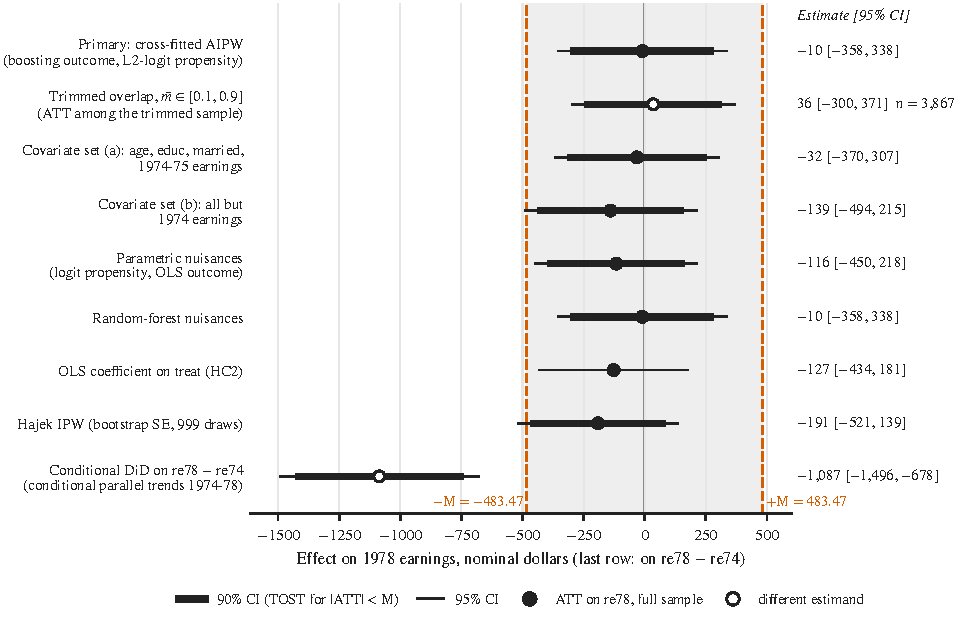
\includegraphics[width=\textwidth]{figures/fig_forest.pdf}
\caption{Primary estimate and every planned robustness estimate, with the equivalence margin.
Each row is one specification, in the order of the analysis plan. The dot is the point
estimate, the thick bar the 90\% confidence interval (the interval of the equivalence test)
and the thin bar the 95\% interval. The OLS row has no thick bar, because no 90\% interval
was logged for OLS. The dashed lines and gray band mark $\pm M$, $M = \EquivMargin$ dollars,
fixed before any outcome column was read; the solid gray line marks zero. Filled dots are ATTs on
1978 earnings in the full sample of $\PrimaryN$. Open dots are different estimands: the
trimmed-overlap ATT over the $\TrimN$ people with $\bar m \in [0.1, 0.9]$, and the
conditional difference-in-differences ATT on re78 $-$ re74 under conditional parallel trends
from 1974 to 1978, with time-invariant covariates only. The latter ($\DiffSeventyFourEffect$,
95\% CI \ci{\DiffSeventyFourCILow}{\DiffSeventyFourCIHigh}) rejects zero and lies outside
$\pm M$; its bias is upward if enrolees' 1974 earnings were already transitorily depressed
and downward if they were on a permanently lower growth path, and the runs cannot tell these
apart. The right column prints each estimate and its 95\% CI, rounded to dollars. Standard
errors are influence-function based for the AIPW rows, HC2 for OLS and a 999-draw bootstrap
for the Hajek IPW. The descriptive \texttt{select-re75} contrast is not an estimate of this
ATT and is not plotted (Table~\ref{tab:main}, panel B).}
\label{fig:forest}
\end{figure}

\section{Sensitivity to unobserved confounding}
\label{sec:sensitivity}

\paragraph{Model.} \citet{imbens2003} studies how sensitive program-evaluation estimates are
to departures from unconfoundedness. We verified that source from its opening text only,
which states this aim, so we cite it for the aim and not for the details below. The model
is the one specified in the plan, which calls it the Imbens model; we use that name without
claiming that it matches Imbens's specification in every detail. It posits a binary confounder
$U \sim \text{Bernoulli}(0.5)$, independent of $X$, with
\[
\operatorname{logit} P(D = 1 \mid X, U) = \gamma' B(X) + \alpha U, \qquad
\var{re78} = \tau D + \beta' B(X) + \delta U + \varepsilon, \quad
\varepsilon \sim N(0, \sigma^2),
\]
and a constant treatment effect, fitted by EM for each fixed $(\alpha, \delta)$. The
confounder's strength is measured by two partial $R^2$s defined before fitting:
$R^2_D = (\alpha^2/4)/(\alpha^2/4 + \pi^2/3)$, its share of the residual latent-index variance
of enrolment, and $R^2_Y = (\delta^2/4)/\sigma_0^2$, its share of the residual variance of
\var{re78} in the $U$-free regression, whose residual SD is $\sigma_0 = \SensSigmaZero$. The
bias of a confounder is $\tau(\alpha, \delta) - \tau(0, 0)$. It is computed within this
parametric model and transferred additively to the AIPW estimate. \textbf{This transfer is an
approximation}, as the plan states: the model's $U$-free estimate $\tau(0, 0) = \SensTauZero$
(which equals the OLS coefficient) differs from the AIPW estimate $\PrimaryEffect$.

\paragraph{Targets and benchmarks.} Three targets were fixed: $t_M = M$; $t_0$, the shift
that would move the nearer 95\% bound to zero and so flip the H1 decision; and $t_E$, the
shift that would end equivalence. For each, $R^2_*$ is the smallest common value
$R^2_D = R^2_Y$ at which $|$bias$|$ reaches the target for either sign of $\delta$. To make
these strengths interpretable, each of nine groups of observed covariates is dropped from
$B(X)$ in turn, and the confounder is placed at the $(R^2_D, R^2_Y)$ that the group's
omission implies. The pre-specified reading rule calls the conclusion for a target robust
to a confounder as strong as a group if $|$bias$|$ at that group's point is below the target
for both signs, and it requires the paper always to state the verdict for the 1975-earnings
group, because an unobserved 1976 shock is plausibly at least as strongly related to
enrolment as the 1975 shock.

\paragraph{Results.} Table~\ref{tab:sensitivity} and Figure~\ref{fig:sensitivity} report the
analysis. The breakdown points are small: $R^2_* = \SensRsqMargin$ for $t_M =
\SensTargetMargin$ dollars, $\SensRsqZero$ for $t_0 = \SensTargetZero$, and $\SensRsqEquiv$
for $t_E = \SensTargetEquiv$. Both observed earnings groups exceed these values in the outcome
equation, and the 1975 group also exceeds them in the enrolment equation: dropping
\var{re75}, its square and \var{unemp75} implies $R^2_D = \SensBenchEarnSeventyFiveRsqD$ and
$R^2_Y = \SensBenchEarnSeventyFiveRsqY$, and a confounder that strong produces $|$bias$|$
$\SensBenchEarnSeventyFiveBias$ dollars.

The reading rule's verdicts are as follows. None of the three conclusions (a shift of the
estimate by $M$, the H1 non-rejection, and the H1b equivalence) is robust to an unobserved
confounder as strong as earnings75. The result could therefore be produced by unobserved
selection of that strength, and an unobserved 1976 earnings shock is plausibly at least that
strongly related to enrolment. For $t_M$ and $t_0$ the conclusion is robust to every other
group, the strongest being earnings74 ($|$bias$|$ $\SensBenchEarnSeventyFourBias$); the
weakest group to which it is not robust is earnings75. For the equivalence target $t_E$ the
conclusion is also not robust to earnings74 ($\SensBenchEarnSeventyFourBias$ against
$\SensTargetEquiv$); it is robust to age ($\SensBenchAgeBias$), schooling
($\SensBenchEducBias$), marriage, the health indicator, urban residence, children and region.
Two qualifications apply to that earnings74 verdict. First, it holds by less than the gap
between the Imbens model's $U$-free estimate and the AIPW estimate, so it lies within the
approximation error of the additive transfer; the rule's verdict stands as written. The
earnings75 verdicts, by contrast, hold by wide margins. Second, the plan did not fix how
groups are ranked when naming the strongest robust and weakest non-robust groups. The code,
written before any analysis run read an outcome value, ranks them by the larger $|$bias$|$ of the two signs at
each group's benchmark point. Under that ranking age is the strongest group to which the
equivalence conclusion is robust; ranking by $R^2_D$ would name schooling instead, and the
two are nearly tied in $|$bias$|$. We therefore list every group.

\begin{table}[tbp]
\centering
\caption{Sensitivity analysis for the primary estimate (the binary-confounder model of
Section~\ref{sec:sensitivity}). Panel A lists the
three planned targets and the diagonal breakdown point $R^2_*$, the smallest
$R^2_D = R^2_Y$ at which $|$bias$|$ reaches the target for either sign, interpolated
linearly between diagonal points. Panel B lists the nine benchmark covariate groups. For each
group, $R^2_D$ and $R^2_Y$ are the strengths implied by dropping the group from $B(X)$, and
$|$bias$|$ is the larger of the two signs from the EM fit at that point. The conclusion for a
target is robust to a group if $|$bias$|$ is below the target for both signs. The
conclusion is not robust to a confounder as strong as earnings75 for any target, so
unobserved selection of that strength could produce the result. For $t_E$ it is also not
robust to earnings74; that verdict ($\SensBenchEarnSeventyFourBias$ against
$\SensTargetEquiv$) holds by less than the gap between the Imbens model's $U$-free estimate
and the AIPW estimate, so it lies within the approximation error. Groups are ordered as in
the plan; age and educ nearly tie in $|$bias$|$. $n = \PrimaryN$.}
\label{tab:sensitivity}
\small
\setlength{\tabcolsep}{4pt}
% Generated by code/tab_sensitivity.py from logged runs. Do not edit by hand; rerun the script.
% Needs \usepackage{booktabs,icomma} and % Generated by `crew.py numbers` from claims.jsonl. Do not edit by hand.
% Each macro is a number taken from a logged run; see claims.jsonl.
\newcommand{\PrimaryEffect}{-10}  % primary-effect
\newcommand{\PrimaryCILow}{-358}  % primary-ci-low
\newcommand{\PrimaryCIHigh}{338}  % primary-ci-high
\newcommand{\PrimarySE}{178}  % primary-se
\newcommand{\PrimaryP}{0.956}  % primary-p
\newcommand{\PrimaryCINinetyLow}{-302}  % primary-ci90-low
\newcommand{\PrimaryCINinetyHigh}{282}  % primary-ci90-high
\newcommand{\PrimaryTOSTP}{0.004}  % primary-tost-p
\newcommand{\PrimaryMinMargin}{302}  % primary-min-margin
\newcommand{\EquivMargin}{483.47}  % equiv-margin
\newcommand{\PrimaryRelEffect}{-0.1}  % primary-rel-effect
\newcommand{\PrimaryRelCILow}{-4.3}  % primary-rel-ci-low
\newcommand{\PrimaryRelCIHigh}{4.1}  % primary-rel-ci-high
\newcommand{\PrimaryCFMean}{7,940}  % primary-cf-mean
\newcommand{\PrimaryTreatedMean}{7,930}  % primary-treated-mean
\newcommand{\PrimaryEffectOverMargin}{-0.02}  % primary-effect-over-margin
\newcommand{\PrimaryN}{4,000}  % primary-n
\newcommand{\PrimaryNTreated}{1,621}  % primary-n-treated
\newcommand{\PrimaryNControl}{2,379}  % primary-n-control
\newcommand{\PrimaryNClipped}{0}  % primary-n-clipped
\newcommand{\OverlapShareOutside}{0.033}  % overlap-share-outside
\newcommand{\OverlapTreatedAboveNineTenths}{0.000}  % overlap-treated-above-09
\newcommand{\SecEarnNextEffect}{-112}  % sec-re79-effect
\newcommand{\SecEarnNextSE}{196}  % sec-re79-se
\newcommand{\SecEarnNextCILow}{-495}  % sec-re79-ci-low
\newcommand{\SecEarnNextCIHigh}{272}  % sec-re79-ci-high
\newcommand{\SecEarnNextP}{0.568}  % sec-re79-p
\newcommand{\SecEarnNextPRW}{0.744}  % sec-re79-p-rw
\newcommand{\SecEarnNextMaxTLow}{-596}  % sec-re79-maxt-low
\newcommand{\SecEarnNextMaxTHigh}{373}  % sec-re79-maxt-high
\newcommand{\SecEmployedEffect}{1.0}  % sec-employed78-effect
\newcommand{\SecEmployedSE}{1.4}  % sec-employed78-se
\newcommand{\SecEmployedCILow}{-1.7}  % sec-employed78-ci-low
\newcommand{\SecEmployedCIHigh}{3.7}  % sec-employed78-ci-high
\newcommand{\SecEmployedP}{0.465}  % sec-employed78-p
\newcommand{\SecEmployedPRW}{0.744}  % sec-employed78-p-rw
\newcommand{\SecEmployedMaxTLow}{-2.4}  % sec-employed78-maxt-low
\newcommand{\SecEmployedMaxTHigh}{4.4}  % sec-employed78-maxt-high
\newcommand{\SecHoursEffect}{48.2}  % sec-hours78-effect
\newcommand{\SecHoursSE}{26.3}  % sec-hours78-se
\newcommand{\SecHoursCILow}{-3.4}  % sec-hours78-ci-low
\newcommand{\SecHoursCIHigh}{99.8}  % sec-hours78-ci-high
\newcommand{\SecHoursP}{0.067}  % sec-hours78-p
\newcommand{\SecHoursPRW}{0.204}  % sec-hours78-p-rw
\newcommand{\SecHoursMaxTLow}{-17.0}  % sec-hours78-maxt-low
\newcommand{\SecHoursMaxTHigh}{113.5}  % sec-hours78-maxt-high
\newcommand{\SecBenefitsEffect}{87}  % sec-benefits78-effect
\newcommand{\SecBenefitsSE}{43}  % sec-benefits78-se
\newcommand{\SecBenefitsCILow}{3}  % sec-benefits78-ci-low
\newcommand{\SecBenefitsCIHigh}{171}  % sec-benefits78-ci-high
\newcommand{\SecBenefitsP}{0.044}  % sec-benefits78-p
\newcommand{\SecBenefitsPRW}{0.166}  % sec-benefits78-p-rw
\newcommand{\SecBenefitsMaxTLow}{-20}  % sec-benefits78-maxt-low
\newcommand{\SecBenefitsMaxTHigh}{194}  % sec-benefits78-maxt-high
\newcommand{\SecWellbeingEffect}{0.06}  % sec-wellbeing78-effect
\newcommand{\SecWellbeingSE}{0.07}  % sec-wellbeing78-se
\newcommand{\SecWellbeingCILow}{-0.08}  % sec-wellbeing78-ci-low
\newcommand{\SecWellbeingCIHigh}{0.21}  % sec-wellbeing78-ci-high
\newcommand{\SecWellbeingP}{0.383}  % sec-wellbeing78-p
\newcommand{\SecWellbeingPRW}{0.744}  % sec-wellbeing78-p-rw
\newcommand{\SecWellbeingMaxTLow}{-0.12}  % sec-wellbeing78-maxt-low
\newcommand{\SecWellbeingMaxTHigh}{0.24}  % sec-wellbeing78-maxt-high
\newcommand{\SecMaxTCrit}{2.477}  % sec-maxt-crit
\newcommand{\SecNDetected}{0}  % sec-n-detected
\newcommand{\SecWellbeingEffectSD}{0.036}  % sec-wellbeing78-effect-sd
\newcommand{\SecWellbeingControlSD}{1.78}  % sec-wellbeing78-control-sd
\newcommand{\SelectEarnPriorEffect}{-3,541}  % select-re75-effect
\newcommand{\SelectEarnPriorCILow}{-3,878}  % select-re75-ci-low
\newcommand{\SelectEarnPriorCIHigh}{-3,204}  % select-re75-ci-high
\newcommand{\SelectEarnPriorOverMargin}{-7.3}  % select-re75-over-margin
\newcommand{\TrimEffect}{36}  % trim-effect
\newcommand{\TrimCILow}{-300}  % trim-ci-low
\newcommand{\TrimCIHigh}{371}  % trim-ci-high
\newcommand{\TrimN}{3,867}  % trim-n
\newcommand{\TrimCINinetyLow}{-246}  % trim-ci90-low
\newcommand{\TrimCINinetyHigh}{317}  % trim-ci90-high
\newcommand{\CovsetAEffect}{-32}  % covset-a-effect
\newcommand{\CovsetACILow}{-370}  % covset-a-ci-low
\newcommand{\CovsetACIHigh}{307}  % covset-a-ci-high
\newcommand{\CovsetAN}{4,000}  % covset-a-n
\newcommand{\CovsetACINinetyLow}{-316}  % covset-a-ci90-low
\newcommand{\CovsetACINinetyHigh}{253}  % covset-a-ci90-high
\newcommand{\CovsetBEffect}{-139}  % covset-b-effect
\newcommand{\CovsetBCILow}{-494}  % covset-b-ci-low
\newcommand{\CovsetBCIHigh}{215}  % covset-b-ci-high
\newcommand{\CovsetBN}{4,000}  % covset-b-n
\newcommand{\CovsetBCINinetyLow}{-437}  % covset-b-ci90-low
\newcommand{\CovsetBCINinetyHigh}{158}  % covset-b-ci90-high
\newcommand{\LearnerLinearEffect}{-116}  % learner-linear-effect
\newcommand{\LearnerLinearCILow}{-450}  % learner-linear-ci-low
\newcommand{\LearnerLinearCIHigh}{218}  % learner-linear-ci-high
\newcommand{\LearnerLinearN}{4,000}  % learner-linear-n
\newcommand{\LearnerLinearCINinetyLow}{-396}  % learner-linear-ci90-low
\newcommand{\LearnerLinearCINinetyHigh}{165}  % learner-linear-ci90-high
\newcommand{\LearnerRFEffect}{-10}  % learner-rf-effect
\newcommand{\LearnerRFCILow}{-358}  % learner-rf-ci-low
\newcommand{\LearnerRFCIHigh}{338}  % learner-rf-ci-high
\newcommand{\LearnerRFN}{4,000}  % learner-rf-n
\newcommand{\LearnerRFCINinetyLow}{-302}  % learner-rf-ci90-low
\newcommand{\LearnerRFCINinetyHigh}{282}  % learner-rf-ci90-high
\newcommand{\DiffSeventyFourEffect}{-1,087}  % diff74-effect
\newcommand{\DiffSeventyFourCILow}{-1,496}  % diff74-ci-low
\newcommand{\DiffSeventyFourCIHigh}{-678}  % diff74-ci-high
\newcommand{\DiffSeventyFourN}{4,000}  % diff74-n
\newcommand{\DiffSeventyFourCINinetyLow}{-1,430}  % diff74-ci90-low
\newcommand{\DiffSeventyFourCINinetyHigh}{-743}  % diff74-ci90-high
\newcommand{\OLSEffect}{-127}  % ols-effect
\newcommand{\OLSCILow}{-434}  % ols-ci-low
\newcommand{\OLSCIHigh}{181}  % ols-ci-high
\newcommand{\OLSN}{4,000}  % ols-n
\newcommand{\IPWEffect}{-191}  % ipw-effect
\newcommand{\IPWCILow}{-521}  % ipw-ci-low
\newcommand{\IPWCIHigh}{139}  % ipw-ci-high
\newcommand{\IPWN}{4,000}  % ipw-n
\newcommand{\IPWCINinetyLow}{-468}  % ipw-ci90-low
\newcommand{\IPWCINinetyHigh}{86}  % ipw-ci90-high
\newcommand{\TrimNTreated}{1,611}  % trim-n-treated
\newcommand{\TrimNDropped}{133}  % trim-n-dropped
\newcommand{\SensRsqMargin}{0.060}  % sens-r2-margin
\newcommand{\SensTargetMargin}{483}  % sens-target-margin
\newcommand{\SensRsqZero}{0.042}  % sens-r2-zero
\newcommand{\SensTargetZero}{338}  % sens-target-zero
\newcommand{\SensRsqEquiv}{0.023}  % sens-r2-equiv
\newcommand{\SensTargetEquiv}{181}  % sens-target-equiv
\newcommand{\SensBenchAgeRsqD}{0.010}  % sens-bench-age-r2d
\newcommand{\SensBenchAgeRsqY}{0.025}  % sens-bench-age-r2y
\newcommand{\SensBenchAgeBias}{128}  % sens-bench-age-bias
\newcommand{\SensBenchEducRsqD}{0.024}  % sens-bench-educ-r2d
\newcommand{\SensBenchEducRsqY}{0.010}  % sens-bench-educ-r2y
\newcommand{\SensBenchEducBias}{126}  % sens-bench-educ-bias
\newcommand{\SensBenchMarriedRsqD}{0.000}  % sens-bench-married-r2d
\newcommand{\SensBenchMarriedRsqY}{0.001}  % sens-bench-married-r2y
\newcommand{\SensBenchMarriedBias}{6}  % sens-bench-married-bias
\newcommand{\SensBenchUrbanRsqD}{0.000}  % sens-bench-urban-r2d
\newcommand{\SensBenchUrbanRsqY}{0.001}  % sens-bench-urban-r2y
\newcommand{\SensBenchUrbanBias}{5}  % sens-bench-urban-bias
\newcommand{\SensBenchRegionRsqD}{0.000}  % sens-bench-region-r2d
\newcommand{\SensBenchRegionRsqY}{0.000}  % sens-bench-region-r2y
\newcommand{\SensBenchRegionBias}{0}  % sens-bench-region-bias
\newcommand{\SensBenchChildrenRsqD}{0.000}  % sens-bench-children-r2d
\newcommand{\SensBenchChildrenRsqY}{0.000}  % sens-bench-children-r2y
\newcommand{\SensBenchChildrenBias}{1}  % sens-bench-children-bias
\newcommand{\SensBenchHealthRsqD}{0.002}  % sens-bench-health-r2d
\newcommand{\SensBenchHealthRsqY}{0.000}  % sens-bench-health-r2y
\newcommand{\SensBenchHealthBias}{6}  % sens-bench-health-bias
\newcommand{\SensBenchEarnSeventyFourRsqD}{0.010}  % sens-bench-earn74-r2d
\newcommand{\SensBenchEarnSeventyFourRsqY}{0.066}  % sens-bench-earn74-r2y
\newcommand{\SensBenchEarnSeventyFourBias}{204}  % sens-bench-earn74-bias
\newcommand{\SensBenchEarnSeventyFiveRsqD}{0.189}  % sens-bench-earn75-r2d
\newcommand{\SensBenchEarnSeventyFiveRsqY}{0.237}  % sens-bench-earn75-r2y
\newcommand{\SensBenchEarnSeventyFiveBias}{1,716}  % sens-bench-earn75-bias
\newcommand{\SensTauZero}{-127}  % sens-tau00
\newcommand{\SensSigmaZero}{4,407}  % sens-sigma-zero
\newcommand{\MissingEarnTreated}{0}  % missing-re78-treated
\newcommand{\InvalidEarnTreated}{0}  % invalid-re78-treated
\newcommand{\MissingEarnControl}{0}  % missing-re78-control
\newcommand{\InvalidEarnControl}{0}  % invalid-re78-control
\newcommand{\MissingEarnNextTreated}{0}  % missing-re79-treated
\newcommand{\InvalidEarnNextTreated}{0}  % invalid-re79-treated
\newcommand{\MissingEarnNextControl}{0}  % missing-re79-control
\newcommand{\InvalidEarnNextControl}{0}  % invalid-re79-control
\newcommand{\MissingEmployedTreated}{0}  % missing-employed78-treated
\newcommand{\InvalidEmployedTreated}{0}  % invalid-employed78-treated
\newcommand{\MissingEmployedControl}{0}  % missing-employed78-control
\newcommand{\InvalidEmployedControl}{0}  % invalid-employed78-control
\newcommand{\MissingHoursTreated}{0}  % missing-hours78-treated
\newcommand{\InvalidHoursTreated}{0}  % invalid-hours78-treated
\newcommand{\MissingHoursControl}{0}  % missing-hours78-control
\newcommand{\InvalidHoursControl}{0}  % invalid-hours78-control
\newcommand{\MissingBenefitsTreated}{0}  % missing-benefits78-treated
\newcommand{\InvalidBenefitsTreated}{0}  % invalid-benefits78-treated
\newcommand{\MissingBenefitsControl}{0}  % missing-benefits78-control
\newcommand{\InvalidBenefitsControl}{0}  % invalid-benefits78-control
\newcommand{\MissingWellbeingTreated}{0}  % missing-wellbeing78-treated
\newcommand{\InvalidWellbeingTreated}{0}  % invalid-wellbeing78-treated
\newcommand{\MissingWellbeingControl}{0}  % missing-wellbeing78-control
\newcommand{\InvalidWellbeingControl}{0}  % invalid-wellbeing78-control
 for the macros
% (icomma keeps the thousands comma in math mode, e.g. $1,716$, without a space).
\begin{tabular}{@{}l l r r r c c c@{}}
\toprule
\multicolumn{8}{@{}l}{\emph{A. Targets and the diagonal breakdown point}} \\
\multicolumn{4}{@{}l}{Target} & Value (\$) & \multicolumn{3}{c}{$R^2_*$ ($R^2_D = R^2_Y$)} \\
\midrule
\multicolumn{4}{@{}l}{$t_M = M$: shift that would move the estimate to the margin} & $\SensTargetMargin$ & \multicolumn{3}{c}{$\SensRsqMargin$} \\
\multicolumn{4}{@{}l}{$t_0$: shift that would move the nearer 95\% bound to zero (flips H1)} & $\SensTargetZero$ & \multicolumn{3}{c}{$\SensRsqZero$} \\
\multicolumn{4}{@{}l}{$t_E$: shift that would end equivalence (90\% CI leaves $\pm M$)} & $\SensTargetEquiv$ & \multicolumn{3}{c}{$\SensRsqEquiv$} \\
\midrule
\multicolumn{8}{@{}l}{\emph{B. Benchmark covariate groups (a confounder as strong as the group)}} \\
 & & & & & \multicolumn{3}{c}{Robust for target} \\
\cmidrule(l){6-8}
Group & Terms dropped from $B(X)$ & $R^2_D$ & $R^2_Y$ & $|$bias$|$ (\$) & $t_M$ & $t_0$ & $t_E$ \\
\midrule
age & age, age$^2$ & $\SensBenchAgeRsqD$ & $\SensBenchAgeRsqY$ & $\SensBenchAgeBias$ & yes & yes & yes \\
educ & educ, educ$^2$ & $\SensBenchEducRsqD$ & $\SensBenchEducRsqY$ & $\SensBenchEducBias$ & yes & yes & yes \\
married & married & $\SensBenchMarriedRsqD$ & $\SensBenchMarriedRsqY$ & $\SensBenchMarriedBias$ & yes & yes & yes \\
urban & urban & $\SensBenchUrbanRsqD$ & $\SensBenchUrbanRsqY$ & $\SensBenchUrbanBias$ & yes & yes & yes \\
region & 3 region dummies & $\SensBenchRegionRsqD$ & $\SensBenchRegionRsqY$ & $\SensBenchRegionBias$ & yes & yes & yes \\
children & children & $\SensBenchChildrenRsqD$ & $\SensBenchChildrenRsqY$ & $\SensBenchChildrenBias$ & yes & yes & yes \\
health\_limit & health\_limit & $\SensBenchHealthRsqD$ & $\SensBenchHealthRsqY$ & $\SensBenchHealthBias$ & yes & yes & yes \\
earnings74 & re74, re74$^2$, unemp74 & $\SensBenchEarnSeventyFourRsqD$ & $\SensBenchEarnSeventyFourRsqY$ & $\SensBenchEarnSeventyFourBias$ & yes & yes & no \\
earnings75 & re75, re75$^2$, unemp75 & $\SensBenchEarnSeventyFiveRsqD$ & $\SensBenchEarnSeventyFiveRsqY$ & $\SensBenchEarnSeventyFiveBias$ & no & no & no \\
\midrule
\multicolumn{8}{@{}l}{U-free estimate in the Imbens model: $\tau(0,0) = \SensTauZero$ (equals the OLS coefficient);} \\
\multicolumn{8}{@{}l}{AIPW estimate $\PrimaryEffect$; residual SD of the U-free outcome model $\sigma_0 = \SensSigmaZero$.} \\
\multicolumn{8}{@{}l}{$|$bias$|$ is computed within the Imbens model and transferred} \\
\multicolumn{8}{@{}l}{additively to the AIPW estimate as an approximation.} \\
\bottomrule
\end{tabular}

\end{table}

\begin{figure}[tbp]
\centering
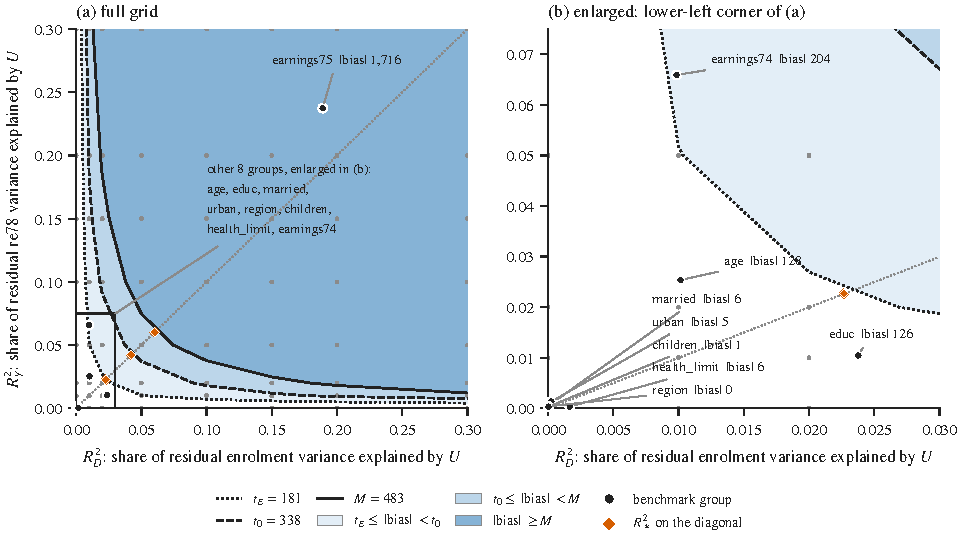
\includegraphics[width=\textwidth]{figures/fig_sensitivity.pdf}
\caption{Sensitivity of the primary estimate to an unobserved binary confounder $U$ (the
model of Section~\ref{sec:sensitivity}). The horizontal axis is $R^2_D$, the share of the residual latent
variance of enrolment explained by $U$; the vertical axis is $R^2_Y$, the share of the
residual variance of re78 explained by $U$. Shading and contour lines show the larger
$|$bias$|$ of the two signs of $U$'s outcome effect, from the EM fits on the planned grid
(gray dots), interpolated linearly between grid points. The dotted line is
$t_E = \SensTargetEquiv$ dollars, the shift that would end equivalence; the dashed line is
$t_0 = \SensTargetZero$, the shift that would move the nearer 95\% bound to zero; the solid
line is $M = \SensTargetMargin$. Orange diamonds on the dotted diagonal ($R^2_D = R^2_Y$) are
the breakdown points $\SensRsqEquiv$, $\SensRsqZero$ and $\SensRsqMargin$. Black dots are the
nine benchmark covariate groups, each placed at the strength that dropping it from $B(X)$
implies; panel (a) shows the full grid and panel (b) enlarges its lower-left corner, where
eight of the nine groups lie. The $|$bias$|$ printed next to each group is the EM fit at that
point. A confounder as strong as earnings75 ($|$bias$|$ $\SensBenchEarnSeventyFiveBias$)
exceeds every target, so the conclusion is not robust to unobserved selection of that
strength; one as strong as earnings74 ($\SensBenchEarnSeventyFourBias$) exceeds $t_E$ only.
The bias is computed within the parametric model and transferred additively to the AIPW
estimate as an approximation; the model's $U$-free estimate is $\SensTauZero$ against the
AIPW estimate of $\PrimaryEffect$, and the earnings74 verdict for $t_E$ holds by less than
this gap. $n = \PrimaryN$.}
\label{fig:sensitivity}
\end{figure}

\FloatBarrier
\section{Limitations}
\label{sec:limitations}

\begin{itemize}
\item \textbf{The identifying assumption is untested and fragile.} The design has no
informative falsification test. The pre-program dip, the unobserved 1976 shock, and the
sensitivity analysis together mean that the equivalence result could be produced by
unobserved selection as strong as the observed selection on 1975 earnings. The conditional
difference-in-differences estimate, under a different assumption, lies far below $-M$, and
the data cannot say which assumption is closer to the truth.
\item \textbf{The sensitivity analysis is approximate.} Its bias is computed in a parametric
linear-outcome, logit-treatment model with a binary confounder and a constant effect, and
added to a nonparametric AIPW estimate. The earnings74 verdict for equivalence lies within
the error of that approximation. The benchmark strengths for each group come from dropping
observed covariates, which says how strong a confounder would be if it resembled them, not
how strong the actual omitted variables are.
\item \textbf{Omitted variables.} Beyond the 1976 shock, motivation, local labour markets
finer than region and urban residence, and whatever the twenty undocumented survey items
measure are all omitted. The survey items were excluded because their timing is unknown; if
they are pre-program measures of motivation, leaving them out weakens unconfoundedness.
\item \textbf{The margin is the crew's choice.} $M$ is 10\% of enrolees' mean 1975 earnings,
which the dip depresses. A margin anchored on 1974 earnings would be larger. No external
benchmark supports 10\%.
\item \textbf{Units and scales.} No price year is documented, so earnings are nominal; the
well-being scale is assumed to be integer 0--10; the treatment records enrolment, not
completion.
\item \textbf{Horizon.} The primary outcome is measured roughly a year after the program.
Training effects are typically close to zero in the short run and larger two to three years
later \citep{card2018}; \var{re79} extends the horizon by one year only.
\item \textbf{Synthetic data.} The results describe this synthetic extract. They are not
evidence about any real program, and no policy claim follows from them.
\end{itemize}

\section{Deviations from the approved design and disclosures}
\label{sec:deviations}

\paragraph{Deviations.} Two, neither of which changes any reported number or decision.
(a)~The Hajek IPW propensity was clipped to $[0.01, 0.99]$; the plan specifies clipping only
for the primary estimator. No unit was clipped in the full-sample fit; clipping in the
bootstrap draws was not counted.
(b)~The plan's rule that H1b also requires the trimmed-overlap 90\% interval inside $\pm M$
if overlap rule O1 or O2 fails was not coded. It was dormant, because both rules passed in
the primary run, and the trimmed 90\% interval \ci{\TrimCINinetyLow}{\TrimCINinetyHigh} lies
inside $\pm M$ in any case.
Otherwise every planned analysis run was executed once, in the planned order, after the
design gate, and none was repeated or replaced. The inverse-probability-of-observation check
was not run because its trigger, fixed and evaluated before the design gate, did not fire.
The design part of the plan was unchanged from the gate to the results; only task statuses
were updated.

\paragraph{Implementation choices and caveats.} (i)~The relative-effect interval, the
Romano--Wolf $p$-values and the max-$t$ intervals use the influence function averaged over
repetitions, as the plan specifies. This omits the between-repetition variance included in
the standard errors, so they are slightly narrower (anti-conservative) than the
standard-error convention would give; no decision depends on it.
(ii)~The plan did not fix how benchmark groups are ranked when naming the strongest robust
and weakest non-robust group in the sensitivity analysis; the ranking was chosen in code
before any analysis run read an outcome value (Section~\ref{sec:sensitivity}).

\paragraph{Process disclosures.}
\begin{itemize}
\item \textbf{The PI held the answer key and set the frame of the study.} The synthetic
dataset's generator and its hidden answer key were written by the same Claude Code session
that acted as PI for this study, so the PI knew the true effect. That session also drafted
the research question and hypotheses, replaced the \$1,000 margin with the 10\%-of-\var{re75}
rule at the Reviewer's suggestion, wrote the pre-gate diagnostics into the plan, issued the
pre-gate rulings that let two runs read the outcome columns, and wrote every brief to the
other agents. The briefs were not archived when they were sent. A reconstruction written by
the PI after the fact (\texttt{briefs/RECONSTRUCTION.md}) says that no brief passed on the
true effect, the generator's structure or the key, and that the PI suggested the admissible
outcome ranges to the Designer; it cannot be verified. The agents that designed and ran the
analysis and wrote this paper did not open the answer key, but that the key did not reach
them through the briefs rests on the PI's word.
\item \textbf{Outcome-blindness rests on the crew's own records.} The full outcome file was
in the workspace from data preparation onward. Two counts-only runs read the outcome columns
before the design gate, and the admissible-range rule was written after the first of them
had run. That no outcome value was analysed before the gate is attested by the code (whose
scripts read the outcome columns only in those two runs and in the analysis runs, apart from
the byte-for-byte copy and hash of the extract), by the run ledger,
by the log and by git history, all kept by the crew itself.
\item \textbf{A PI ruling was logged retroactively.} The PI allowed the missing-value count
in response to a design-review finding (design round 1, finding F4). According to the PI, the
ruling was given in its instructions to the Designer before that count ran; the only record
is the PI's own log entry, written after the count at the Reviewer's request and marked as
retroactive. The ruling for the range count was logged before that count ran.
\item \textbf{The code was reviewed after the runs.} The plan predates the crew's rule that
analysis code is reviewed before any analysis run, so the Reviewer's code review took place
after every analysis run had finished. It passed with four minor findings, which correspond to
deviations (a) and (b) and items (i) and (ii) above. The Reviewer re-implemented the primary
estimator independently and reproduced it, and found that every analysis script was last
modified after the design gate and before the first analysis run. The findings were answered
in the files and judged answered in the second results review, but their status in the
code-review record is still open, and no second code round was held.
\item \textbf{No literature review round was held.} The crew's playbook calls for one before
the design gate. The bibliography was compiled and checked against the sources by the Scout
alone; the Reviewer spot-checked some entries only during the paper review.
\item \textbf{The PI deleted a log entry.} The Scout's hand-written entry recording the end of
the novelty check carried a timestamp in the future. At the Reviewer's request (question
round 1, finding F8) the PI removed it from the append-only log and logged the removal; the
time at which the Scout finished that task is therefore unknown.
\item \textbf{The equivalence margin was revised once}, at the question stage and before any
data were fetched (Section~\ref{sec:data}).
\item \textbf{Repeated data-prep runs.} Two outcome-blind data-preparation runs (covariate
preparation and the margin) were each run twice before the design gate, after a consistency
check on the unemployment indicators was added; the ledger keeps the second run of each.
\end{itemize}

\section{Conclusion}

In this synthetic extract, the pre-specified cross-fitted AIPW estimate of the effect of
enrolment on enrolees' 1978 earnings is $\PrimaryEffect$ dollars, with 95\% interval
\ci{\PrimaryCILow}{\PrimaryCIHigh}. A zero ATT is not rejected. Under unconfoundedness
given the eleven covariates, the effect is smaller in magnitude than the pre-set margin of
$\EquivMargin$ dollars, and no check covered by the pre-specified disagreement rule
overturns this. That conclusion is
not robust to an unobserved confounder as strong as the 1975-earnings covariates, which would
move the estimate by up to $\SensBenchEarnSeventyFiveBias$ dollars: the result could be
produced by unobserved selection of that strength, and an unobserved 1976 earnings shock is
plausibly at least that strongly related to enrolment. The equivalence conclusion is not
robust to a confounder as strong as 1974 earnings either. Under conditional parallel trends
from 1974, the estimate is $\DiffSeventyFourEffect$ dollars. None of the five secondary
outcomes is detected.

The honest summary is an interval and a conditional statement, not a verdict on the
program. Pre-specification did what it is supposed to do here: it kept the outcome list, the
margin and the reading of every check fixed, so the fragility of the result is reported
rather than discovered by a reader. It cannot remove the fragility. Pre-analysis plans have
costs and limits \citep{olken2015,coffman2015}, and the clean rerun of every result and
outside replication remain the stronger correctives. Settling the question would need data
that this extract does not contain: 1976 earnings, or a source of variation in enrolment
unrelated to earnings shocks.

\section*{AI-use statement}

This paper was drafted by a crew of AI research-assistant agents
(Free-Research-Crew, protocol v0.1) under the direction of the human author, Bryce Wang.
He approved the research question, the design and the results at three human gates, and
the manuscript itself is subject to a fourth, the submission gate. He takes responsibility
for the paper's content.

\begin{itemize}
  \item \textbf{Roles and models.} Every crew role ran on Anthropic Claude through Claude
        Code. The PI role was the main Claude Code session. The Scout, Designer, Data RA,
        Econometrician, Figures RA, Reviewer and Writer ran as subagents launched from that
        session. The review records name the model as \texttt{claude-opus-5-5}. The
        Replicator role, which reruns every run from a clean environment, had not run when
        this draft was written.
  \item \textbf{Review.} The Reviewer agent ran 3 rounds on the research question, 3 on the
        design, 1 on the code and 2 on the results; the paper review comes before the
        submission gate. Its independence level was \emph{fresh-context}: a new context in
        every round, with the same model family as the other roles. The human author chose
        this over a cross-family reviewer. The code review took place after the analysis
        runs, because the study's plan predates the crew's rule that code is reviewed before
        any analysis run (see Section~\ref{sec:deviations}); it passed with four minor
        findings, all answered in the files and in this paper. The final question round and
        the final results round each passed with two minor findings still open; the human
        approved those gates, and the open findings were then addressed (by the design, and
        by the figures and the approximation wording, respectively).
  \item \textbf{Findings accepted over the Reviewer's objection.} None.
  \item \textbf{Retroactive ruling.} The PI's ruling on design-review finding F4, which
        allowed a pre-gate run to count missing outcome values by arm, was given before
        that run but logged only afterwards, and is marked as retroactive in the log
        (Section~\ref{sec:deviations}).
  \item \textbf{Seed authorship.} The synthetic dataset's generator and its hidden answer
        key were written by the same Claude Code session that acted as PI. The agents that
        analysed the data and wrote the paper never saw the answer key.
  \item \textbf{Evidence.} Every reported number is a macro generated from the metrics of
        a logged run, and none was typed by hand. Every citation was checked against its
        source: 9 from the full text and 14 from the abstract only. Where only the abstract
        could be read, the paper says no more than the abstract does. The clean rerun of
        every run from a fresh environment is pending: no replication record exists yet.
        The full workspace is public at
        \url{https://github.com/brycewang-stanford/Free-Research-Crew/tree/main/gallery/ss-null-effect}.
        It contains the plan, the run ledger, the code, the data manifest, every review and
        this paper's sources.
\end{itemize}


\bibliographystyle{plainnat}
\bibliography{../refs}

\end{document}
